\documentclass{trlnotes}
\usepackage{trmath}
\addcompatiblelayout{commonplace}
\setlayout{commonplace}
% \usepackage{amsthm}
\usepackage{trthm}
\usepackage{trphys}
% \RequirePackage{stmaryrd}

% \RequirePackage{etoolbox}


%\RequirePackage{cmap}
% \RequirePackage{hyperref}
% \theoremstyle{definition}
% \newtheorem{thm}{Теорема}
% \newtheorem{de}{Определение}
% \newtheorem{lm}{Лемма}
% \newtheorem{exm}{Пример}
% \newtheorem{pr}{Свойство}
% \newtheorem{exc}{Упражнение}
% \newtheorem{cor}{Следствие}
% \newtheorem{st}{Утверждение}
% \theoremstyle{remark}
% \newtheorem{rem}{Замечание}
\newcommand*{\icom}{\ensuremath\text{\textit{,}}}
\newcommand*{\icol}{\ensuremath\text{\textit{:}}}
\newcommand*{\iscol}{\ensuremath\text{\textit{;}}}
\newcommand*{\com}{\ensuremath\text{\text{,}}}
\newcommand*{\col}{\ensuremath\text{\text{:}}}
\newcommand*{\scol}{\ensuremath\text{\text{;}}}
% \newcommand*{\so}{\ensuremath\Rightarrow}
\newcommand*{\bso}{\ensuremath\Leftarrow}
\newcommand*{\eqv}{\ensuremath\Leftrightarrow}
\newcommand*{\all}{\forall}
\newcommand*{\ex}{\exists \,}
% \newcommand*{\ov}{\overline}
\newcommand*{\un}{\underline}
\newcommand*{\ova}{\overrightarrow}
\newcommand*{\auth}[1]{\hfill \textit{#1}}
\newcommand*{\pd}{\partial}
% \newcommand*{\R}{\mathbb{R}}
% \newcommand*{\N}{\mathbb{N}}
\newcommand*{\DD}{\mathbb{D}}
\newcommand*{\K}{\mathbb{K}}
% \newcommand*{\C}{\mathbb{C}}
% \newcommand*{\C}{\mathbb{C}}
% \newcommand*{\Q}{\mathbb{Q}}
\newcommand{\An}{\wedge}
\newcommand{\Or}{\vee}
% \newcommand*{\Z}{\mathbb{Z}}
\newcommand*{\J}{\mathbb{J}}
\newcommand*{\bas}[2]{\overset{\vspace{-3pt}\tiny{\mb{#1}}}{#2}}
\newcommand*{\mc}{\mathcal}
\newcommand*{\mb}{\mathbf}
\newcommand*{\mf}{\mathfrak}
\newcommand*{\ti}{\textit}
\newcommand*{\la}{\langle}
\newcommand*{\ra}{\rangle}
\newcommand*{\tb}{\textbf}
\newcommand*{\mr}{\mathrm}
\newcommand*{\wt}{\widetilde}



% \DeclareMathOperator{\rk}{rk}
\DeclareMathOperator{\Dom}{Dom}
% \DeclareMathOperator{\id}{id}
\DeclareMathOperator{\Cl}{Cl}
% \DeclareMathOperator{\Res}{Res}
\DeclareMathOperator{\im}{Im}
% \DeclareMathOperator{\rot}{rot}
\DeclareMathOperator{\Div}{div}
% \DeclareMathOperator{\grad}{grad}
\DeclareMathOperator{\Id}{Id}
% \DeclareMathOperator{\Aut}{Aut}
% \DeclareMathOperator{\Stab}{Stab}
\DeclareMathOperator{\const}{const}

%\titleformat{\section}
%  {\sffamily\mdseries\upshape\LARGE}
%  {Билет \thesection:}{0.5em}{}



\usepackage[normalem]{ulem}
\usepackage{trsym}
\usepackage{docmute}
\usepackage{luacode}
\usepackage{tikz} 
\graphicspath{{img/}}
\title{методы отчислений}
\date{10.01.2019\\
  \small версия от \luaexec{tex.print(os.date("\%d.\%m.\%Y \%X"))}, 
до экзамена
\directlua{tex.print(math.floor(os.difftime(os.time{
day=10, month=1, year=2019, hour=11 },os.time())/3600))}
часов}
\author{Лектор: Б.~А.~Самокиш}

\usepackage{luatex85}
\usepackage[all]{xy}
\begin{document}
 
\maketitle
\tableofcontents
\clearpage

\makeatletter
\let \old@to\to \let\to\relax
\let \oldxypicxto \xto
\let \xto\relax
\newcommand\xto[1]{\ensuremath \xrightarrow[#1]{}}
\makeatother
\chapter{Однородные дифференциальные уравнения}
\label{chap:ode}
\documentclass{trlnotes}
\usepackage{trmath}
\addcompatiblelayout{commonplace}
\setlayout{commonplace}
\usepackage{trthm}
\usepackage{trsym} 
\usepackage{trphys}
% % \RequirePackage{stmaryrd}

% \RequirePackage{etoolbox}


%\RequirePackage{cmap}
% \RequirePackage{hyperref}
% \theoremstyle{definition}
% \newtheorem{thm}{Теорема}
% \newtheorem{de}{Определение}
% \newtheorem{lm}{Лемма}
% \newtheorem{exm}{Пример}
% \newtheorem{pr}{Свойство}
% \newtheorem{exc}{Упражнение}
% \newtheorem{cor}{Следствие}
% \newtheorem{st}{Утверждение}
% \theoremstyle{remark}
% \newtheorem{rem}{Замечание}
\newcommand*{\icom}{\ensuremath\text{\textit{,}}}
\newcommand*{\icol}{\ensuremath\text{\textit{:}}}
\newcommand*{\iscol}{\ensuremath\text{\textit{;}}}
\newcommand*{\com}{\ensuremath\text{\text{,}}}
\newcommand*{\col}{\ensuremath\text{\text{:}}}
\newcommand*{\scol}{\ensuremath\text{\text{;}}}
% \newcommand*{\so}{\ensuremath\Rightarrow}
\newcommand*{\bso}{\ensuremath\Leftarrow}
\newcommand*{\eqv}{\ensuremath\Leftrightarrow}
\newcommand*{\all}{\forall}
\newcommand*{\ex}{\exists \,}
% \newcommand*{\ov}{\overline}
\newcommand*{\un}{\underline}
\newcommand*{\ova}{\overrightarrow}
\newcommand*{\auth}[1]{\hfill \textit{#1}}
\newcommand*{\pd}{\partial}
% \newcommand*{\R}{\mathbb{R}}
% \newcommand*{\N}{\mathbb{N}}
\newcommand*{\DD}{\mathbb{D}}
\newcommand*{\K}{\mathbb{K}}
% \newcommand*{\C}{\mathbb{C}}
% \newcommand*{\C}{\mathbb{C}}
% \newcommand*{\Q}{\mathbb{Q}}
\newcommand{\An}{\wedge}
\newcommand{\Or}{\vee}
% \newcommand*{\Z}{\mathbb{Z}}
\newcommand*{\J}{\mathbb{J}}
\newcommand*{\bas}[2]{\overset{\vspace{-3pt}\tiny{\mb{#1}}}{#2}}
\newcommand*{\mc}{\mathcal}
\newcommand*{\mb}{\mathbf}
\newcommand*{\mf}{\mathfrak}
\newcommand*{\ti}{\textit}
\newcommand*{\la}{\langle}
\newcommand*{\ra}{\rangle}
\newcommand*{\tb}{\textbf}
\newcommand*{\mr}{\mathrm}
\newcommand*{\wt}{\widetilde}



% \DeclareMathOperator{\rk}{rk}
\DeclareMathOperator{\Dom}{Dom}
% \DeclareMathOperator{\id}{id}
\DeclareMathOperator{\Cl}{Cl}
% \DeclareMathOperator{\Res}{Res}
\DeclareMathOperator{\im}{Im}
% \DeclareMathOperator{\rot}{rot}
\DeclareMathOperator{\Div}{div}
% \DeclareMathOperator{\grad}{grad}
\DeclareMathOperator{\Id}{Id}
% \DeclareMathOperator{\Aut}{Aut}
% \DeclareMathOperator{\Stab}{Stab}
\DeclareMathOperator{\const}{const}

%\titleformat{\section}
%  {\sffamily\mdseries\upshape\LARGE}
%  {Билет \thesection:}{0.5em}{}



\usepackage{silence}
\WarningFilter{latex}{Reference}
\graphicspath{{../../img/}}
\newtagform{roman}[\renewcommand{\theequation}{\Roman{equation}}]()
\begin{document}
\paragraph{Краевая задача для ОДУ 2 порядка и сведение к задаче Коши}
\label{par:ode::bprobl}
\begin{defn}\label{defn:ode::bprobl}
  Рассмотрим ОДУ 2 порядка
  \[
    y'' + p(x) y' + q(x) y = f(x) \qquad y \in C^2([a;b])
  \]
  и 3 варианта условий на $y$
  \begin{enumerate}[I]
    \item $y(a) = A, \quad y(b) = B$ \label{it:ode::bprobl::cond:i}
    \item $y'(a) = A, \quad y'(b) = B$ \label{it:ode::bprobl::cond::ii}
    \item $y'(a) = α y(a) + A, \quad y'(b) = βy(b) + B$ \label{it:ode::bprobl::cond::iii}
    \end{enumerate}
  
  Если $y$~--- решение для которого выполнено какое-то из условий выше, то $y$~--- решение
  граничной задачи.
\end{defn}

\begin{defn}[Однородная краевая задача]\label{defn:ode::bprobl::hom}
  Положим $f \equiv 0$ в \ref{defn:ode::bprobl}.
\end{defn}
\begin{defn}[Однородные граничные условия]\label{defn:ode::bprobl::hombnd}
  Положим $A = B = 0$ в граничных условиях в \ref{defn:ode::bprobl}
\end{defn}

\begin{thrm}[об альтернативе]\label{thrm:ode::bprobl::alt}
  Рассмотрим однородную граничную задачу с однородными граничными условиями.
  Пусть $y_H$~--- решение однородной задачи. 

  Тогда
  \begin{enumerate}
    \item $y_0 \equiv 0$~--- единственное решение однородной задачи \so неоднородная краевая 
      задача имеет единственное решение
    \item $y_0 \equiv 0$~--- неединственное решение однородной задачи \so неоднородная краевая 
      задача имеет бесконечно много или не имеет решений вовсе
  \end{enumerate}
\end{thrm}


\begin{prf}
  Рассмотреть решение неоднородной краевой в виде $y(x) = y_0(x) + c_1 y_1(x) + c_2 y_2(x)$
  и подставить граничные условия, а дальше все следует из линейной алгебры.
\end{prf}


Разберёмся как численно найти $y_0, y_1, y_2$, потребовавшиеся в предыдущем доказательстве.
Будем считать что $p,q,f$ определены на $I \ni [a;b]$, так что $y$ можно продолжить 
на $(a-ε;b+ε)$. 
\begin{enumerate}
  \item $y(a) = 0$, $y'(a) = 0$. Поскольку $0$ явно решение однородной задачи, то что мы
    найдем будет как раз частным решением неоднородной задачи (Коши!).
  \item $y_H(a) = 1$, $y'_H(a) = 0$ и решаем мы тут однородную задачу (Коши!). Будем считать то что
    нашлось $y_1$
  \item $y_H(a) = 0$, $y'_H(a) = 1$. Скажем что это $y_2$. Здесь важно заметить про линейную
    независимость $y_1$ и $y_2$. Найдем определитель Вронского в точке $a$
    \[
      W = \begin{vmatrix}
        y_1(a) & y_2(a) \\
        y_1'(a) & y_2'(a) 
      \end{vmatrix} = 
      \begin{vmatrix}
        1 & 0 \\ 
        0 & 1 \\
      \end{vmatrix} = 1 \neq 0
    \]
    А тогда он нигде не ноль. А значит $y_1$ и $y_2$ линейно независимы.
\end{enumerate}

Всё это называется \emph{методом начальных данных} для решения краевой задачи.

В рассуждении выше можно было бы взять другие начальные данные дабы
упростить себе жизнь. Ведь никто не запрещает запихать, например, кусок $y_2$ в $y_0$
(если мы уже знаем правильное $c_2$). Нам просто были нужны какие-то линейно независимые
решения однородной задачи.

Рассмотрим граничную задачу в форме \ref{it:ode::bprobl::cond::iii}
\begin{enumerate}
  \item $y(a) = 0$, $y'(a) = A$, нашли  $y_0$.
  \item $y_H(a) = 1$, $y'_H(a) = α$, нашли $y_1$.
  \item $y_H(a) = 0$, $y'_H(a) = 0$. Мы просто решили что $y_2 \equiv 0$. Эту ЗК мы даже
    не решаем, а сразу знаем ответ.
\end{enumerate}
При таком раскладе $y(x) = y_0(x) + c_1 y_1(x)$. 
Проверим левое граничное условие 
\[
  \begin{split}
    y(a) &= y_0(a) + c_1\, y_1(a) = 0 + c_1 \, 1 = c_1 \\
    y'(a) &= y_0'(a) + c_1\, y_1'(a) = A + c_1 \, α = A + α\ y(a)
  \end{split}
\]
Как видно, всё получилось.

В случае \ref{it:ode::bprobl::cond:i} можно сделать так:
\begin{enumerate}
  \item $y(a) = A$, $y'(a) = 0$, нашли $y_0$.
  \item $y_H(a) = 0$, $y_H'(a) = 1$, нашли $y_1$.
\end{enumerate}
Как видно, свободы в выборе $c_1$ хватает чтобы разобраться с правой границей.

\begin{exmp}
  $y'' - q^2 y =0$, $y(0) = 1$, $y(b) = 1$

  \underdev, а он важный вообще-то, из него необходимость метода прогонки следует.
\end{exmp}

\paragraph{Метод дифференциальной прогонки}
\label{par:ode::difftdma}

Здесь будем решать краевую задачу с граничными условиями в форме \ref{it:ode::bprobl::cond::iii}.

Рассмотрим $α(x)$, $β(x) \that$ (прогоночные коэффициенты)
\begin{equation} \label{eq:ode::difftdma::tmda}
  y'(x) = α(x) \, y(x) + β(x)
\end{equation}
Такая форма напрашивается при вспоминании трюка, который мы делали в прошлом параграфе.
Там как раз $y'(a) = y_0(a) + c_1\, y_1(a)$, а $c_1 = y(a)$.
Здесь мы пока вводим прогоночные коэффициенты формально, а существование покажем конструктивно.

Найдем уравнения на $α, β$
\[
  \begin{aligned}
    y'  &= α y + β \\
    y'' &= α y' + α'y + β'
  \end{aligned} \so
  \begin{aligned}[t]
    &y'' + py' + qy = f \\
    \iff &αy' + α'y + β' + p (αy + β) + qy = f \\
    \iff &y\,(\underbrace{α^2 + α' + p α + q}_{0}) + \underbrace{α β + β' + pβ}_f = f 
  \end{aligned}
\]
В итоге получаем систему ОДУ первого порядка
\begin{equation}\label{eq:ode::difftdma::direct}
  \begin{aligned}
    α' &= - α^2 - p α - q \\
    β' &= f - pβ - αβ \\
  \end{aligned}
\end{equation}

Посмотрим что происходит на правом конце\footnote{а что делать если $α(b)=β$ неясно}
\[
  \begin{aligned}
    y'(b) &= α(b) y(b) + β(b) \\
    y'(b) &= β y(b) + B \\
  \end{aligned} \so y(b) = \frac{B- β(b)}{α(b) - β} 
\]
Сам метод выглядит так:
\begin{description}
  \item[прямая прогонка:] решаем систему \eqref{eq:ode::difftdma::direct} с начальными данными
    $α(a) = α$, $β(a) = A$.
  \item[обратная прогонка:] уже зная $α(x)$, $β(x)$ решаем \eqref{eq:ode::difftdma::tmda} c
    начальными данными $y(b) = \frac{B- β(b)}{α(b) - β}$.
\end{description}

\begin{rem}
  Рассмотрим однородную задачу с однородными граничными условиями. 
  Тогда \eqref{eq:ode::difftdma::tmda} переходит в $y'(x) = α(x) \, y(x)$.
  Если при этом $\exists\, c\in (a;b) \that y(c) = 0 \land y'(c) \neq 0$, то $α(c)$ не
  существует. Так что, как видно, не всякое решение краевой задачи можно найти методом
  прогонки.
\end{rem}

\paragraph{Метод прогонки для систем ОДУ}
\label{par:ode::tdmasys}

\begin{defn}\label{defn:ode::tdmasys::bprobl}
  Рассмотрим ОДУ
  \begin{equation}\label{eq:ode::tdmasys::ode}
    \v y' = \hat A(x) \,\v y + \v f(x) \qquad \v y \in C^2([a;b]), \quad y \colon [a;b]\to \R^s
  \end{equation}
  и условия вида
  \begin{equation*}\label{eq:ode::tdmasys::bndcond}
    \begin{aligned}
      x &= a& \hat α \v y(a) &= \v β &\qquad \hat α \colon \R^s \to \R^p \\
      x &= b& \hat γ \v y(b) &= \v δ &\qquad \hat γ \colon \R^s \to \R^q \\
        &   &                &       & s &= p+q
    \end{aligned}
  \end{equation*}
  
  Если $y$~--- решение для которого выполнено условие выше, то $y$~--- решение
  граничной задачи.
\end{defn}

\begin{rem}
  Вообще, граничные условия бывают куда более общего вида, но мы их не рассматриваем.
  То, что у нас~--- это линейные распадающиеся граничные условия.

  А вот так выглядят нераспадающиеся: 
  \[
    \hat α\v y(a) + \hat γ \v y(b) = \v β, \qquad \hat α,\hat γ\colon \R^s\to\R^s
  \]
\end{rem}

Общее решение задачи Коши~\ref{eq:ode::tdmasys::ode} имеет вид
\[
  \v y(x) = \v y_0(x) + \sum_{j=1}^s c_j \v y_j(x)
\]
где как обычно $y_0$~--- решение неоднородной задачи Коши, а $\{y_{j}\}$~--- фундаментальная
система решений однородной.

\clause{Метод начальных данных} такой же в \ref{par:ode::bprobl}~--- находим
из граничных условий $\{c_j\}$ в общем решении.

Чтобы добыть решения задач Коши можно взять $\v y_j(a) = \v e_j$
(это единичный вектор с 1 на $j$ом месте), $\v y_0 (a) =0$

Можно снова уменьшить количество работы
% в этом месте было потеряно больше часа на поиск н.д в явном виде
\begin{enumerate}
  \item в качестве начальных данных для $y_0$~--- какое-нибудь решение системы $\hat α y = β$
  \item в качестве начальных данных для $y_j$, $j\in {p+1}\intrng {s}$~--- $q$ линейно независимых
    решений $\hat αy = 0$
  \item $y_j \equiv 0$, $j \in 1\intrng p$
\end{enumerate}

В итоге решение примет вид 
\[
  \v y(x) = \v y_0 (x) + \sum_{j=p+1}^{s} c_j \v y_j(x) 
\]

\plholdev{здесь снова этот понятный кусок про экспоненты и беды вычислений}\underdev

\clause{Метод прогонки,} в котором cнова зададим $\hat α, \v β$
\begin{equation}\label{eq:ode::tdmasys::tdma}
  \hat α(x) \, \v y(x) = \v β(x),  \qquad \hat α \colon [a;b]×\R^s \to \R^p 
\end{equation}
При таком условии $\forall\, x\holds y(x)\in M \subset \R^s$, $\dim M = s-p$ 
(предполагая что $\rk \hat α(x) = p$) 

Найдем уравнения на $\hat α(x), \v β(x)$
\[\bindvectors{y,β,f}\bindqoperators{α, A}% weeell, they just look simular
  \begin{aligned}
    α y &= β \\
    α y' +  α' y&=  β' \\
  \end{aligned} \so
  \begin{aligned}[t]
    &y' = Ay + f  \\
    &αAy  + αf + α'y  = β' \\
    \iff &(\underbrace{αA + α'})\,y - \underbrace{β'} = - αf 
  \end{aligned}
\]

Пусть $α_j$~--- строка $\hat α$.
Тогда мы получаем систему ОДУ первого порядка
\begin{equation}\label{eq:ode::tdmasys::direct}
  \begin{aligned}
    α_j' &= - \hat A^T \, α_j \\
    β_j' &= (α_j,\v f) \\
  \end{aligned}
\end{equation}

Посмотрим что происходит на правом конце
\begin{equation}\label{eq:ode::tdmasys::rightbndcond}
  \left\{\begin{aligned}
    \hat α(b) \, \v y(b) &= \v β(b) \\
    \hat γ \v y(b) &= \v δ \\
  \end{aligned}\right. 
\end{equation}
это просто линейная система порядка $s$ на $\v y(b)$, решаем и находим.

Сам метод выглядит так:
\begin{description}
  \item[прямая прогонка:] решаем прогоночные уравения\eqref{eq:ode::tdmasys::direct}
    с начальными данными $\hat α(a) = \hat α$, $\v β(a) = \v β$.
  \item[обратная прогонка:] уже зная $α(x)$, $β(x)$ решаем \eqref{eq:ode::tdmasys::tdma} c
    начальными данными $y(b)$, найденным из системы \eqref{eq:ode::tdmasys::rightbndcond}.
\end{description}

\begin{rem}\quest{}
  Метод с заменой $\hat A$ на сопряженную в прогоночных уравениях 
  уже пафосно называется методом \emph{сопряжённых систем}, но ничем кроме
  названия по сути не отличается.
\end{rem}

\begin{rem}
  Вообще, этот метод накладывает слишком жёсткие условия на $\hat α$, $\b β$.
  Например краевая задача из~\ref{par:ode::bprobl} им не решается. 
  Проблема возникает в том месте, где из $(\hat α\hat A + \hat α')\,\v y = 0$ выводится
  $\hat α\hat A + \hat α' =0$. Произвольностью $\v y$ мы вообще-то пользоваться не можем,
  так как на него есть условие $\hat α(x) \, \v y(x) = \v β(x)$.
\end{rem}

\begin{rem}
  У вышеописанного метода есть ещё пара недостатков:
  \begin{enumerate}
    \item $α_j' = -\hat A^T\, α_j$ отличается от исходной системы только отсутствием
      неоднородности, так от проблем связанных с потерей точности из-за собственных
      чисел разного знака в решениях задач Коши мы убежать не смогли.
    \item $\hat α \hat α^T$ может быть плохо обусловленной и ища $\v y(b)$ мы потеряем точность.
      \note{
      $\rk \hat α \hat α^T \geqslant 2\rk \hat α - s$ из теоремы Сильвестра о ранге,
    так что так в одну сторону вроде можно}
  \end{enumerate}

  Собственно, для того чтобы обойти эти проблемы и нужен \ref{par:ode::orthtdma}.
\end{rem}

\paragraph{Ортогональная прогонка}
\label{par:ode::orthtdma}

<<будем решать немного другую задачу>>

Заменим уравенение для $\hat α$ в методе выше.

\[\bindqoperators{α, A}
  α' = - αA \longrightarrow  α' = - α A + αA α^T \left(α α^T\right)^{-1} α
\]

Крокодил в формуле сверху~"--- ортогонанальная проекция $\hat α \hat A$ на $\hat α$,
а скалярное произведение имеет вид $(\hat α, \hat β) = \hat α \hat β^T$\note{
  на самом деле оно несимметрично. Нужно здесь понимать матрицу как набор векторов-строк.
  Тогда какой-то смысл есть.
}.
Так что по идее, раз мы проекцию на $\hat α$ вычли, $(\hat α',\hat α) = 0$.
Проверим:
\[\bindqoperators{α, A}
  α' α^T = -α A α^T + αA α^T \left(α α^T\right)^{-1} αα^T  = -α A α^T + αA α^T = 0
\]
Отсюда следует, что $\fder{}{x} \left( \hat α \hat α^T \right) = 0$, так что
матрица $\hat α \hat α^T$ постоянна на всём $[a;b]$

Получим уравнения на прогоночные коэффициенты
\[\bindvectors{y,β,f}\bindqoperators{α, A}% weeell, they just look simular
  \begin{aligned}[t]
    &αAy  + αf + α'y  = β' \\
    \iff &αAy + αf  -αAy + αAα^T \left(α α^T\right)^{-1} \underbrace{αy}_{β} = β'
  \end{aligned} 
\]
В итоге
\begin{equation}\label{equation:ode::orthtdma::tdma}
  \bindvectors{y,β,f}\bindqoperators{α, A}
  \begin{aligned}
    α' &=  - α A + αA α^T \left(α α^T\right)^{-1} α \\
    β' &= αf + αAα^T \left(α α^T\right)^{-1} β
  \end{aligned} 
\end{equation}

Разберёмся что делать с $\left(α α^T\right)^{-1}$. Не очень приятно каждый раз искать обратную 
матрицу.

На левой границе $\hat α(a) \v y(a) = \v β(a)$. Проведём процесс Грамма-Шмидта и 
ортогонализуем строчки $\hat α(a)$.
При этом заменили переменную в исходном уравении, соответственно поменялись 
$\hat A\to \hat B$, $\v f\to \v g$. Зато $\hat α(a)\, \hat α(a)^T = I$.
Так что прогоночные уравения принимают вид
\begin{equation}\label{equation:ode::orthtdma::tdma}
  \bindvectors{y,β,g}\bindqoperators{α, B}
  \begin{aligned}
    α' &=  - α B + αB α^T α \\
    β' &= αg + αBα^T β
  \end{aligned} 
\end{equation}

Поскольку $\hat α\hat α^T$ постоянна на $[a;b]$ (всюду $I$),
то проблем с её плохой обусловленностью в $x=b$ нет. Правое граничное условие
решится.

Судя по всему, это же условие исключает быстрый рост компонент $\hat α$.
Так что обе проблемы из замечания в конце предыдущего параграфа снимаются.
\quest\note{про это два слова в Крылове написано и больше нигде нет.}

Вышеописанный метод ещё называется методом Абрамова.


\paragraph{Разностный метод для краевой задачи 2 порядка}
\label{par:ode::findiff}
\begin{aux}
  \textit{Предупреждение:}
  в силу повышенной техничности этого параграфа он написан в соответствующем стиле.
  Что поделать. Приятного прочтения.
\end{aux}

Решать краевую задачу для дифференциального уравения второго порядка
\begin{equation}
  y'' + p(x) y' + q(x) y = f(x) \qquad y \in C^2([a;b]) \label{eq:ode::findiff::ode}
\end{equation}

\clause{Алгоритм}
\begin{defn}[Метод разностной прогонки]\label{defn:ode::findiff::alg}
  Пусть задано дифференциальное уравнение с граничными условиями.
  Методом разностной прогонки называет следующий алгоритм:
  \begin{enumerate}
    \item Выбор сетки: узлы, шаг (если она равномерная)
    \item Построение сеточных уравений
      \begin{enumerate}
        \item Диффур в узлах сетки
        \item Все производные через конечные разности
      \end{enumerate}
    \item Решение получившейся линейной системы
  \end{enumerate}
\end{defn}

Будем дальше всюду считать, что решение задано на $[a;b]$
\[
  \text{$n$ узлов}\qquad h = \frac{b-a}{n} \qquad x_k = a + kh
\]
\clause{Формулы численного дифференцирования} 
Здесь $M_n = \max \abs{y^{(m)}(x)}$
\begin{align}
  \label{eq:ode::findiff::simpforward}
  y'(x) &= \frac{y(x+h) -y (x)}{h} + R & \abs{R} &\leqslant \tfrac{hM_2}{2} \\
  \label{eq:ode::findiff::simpbackward}
  y'(x) &= \frac{y(x) - y (x-h)}{h} + R & \abs{R} &\leqslant \tfrac{hM_2}{2} \\
  \label{eq:ode::findiff::threepointforward}
  y'(x) &= \frac{-y(x+2h) + 4y (x+h) - 3y(x)}{2h} + R & \abs{R} &\leqslant \tfrac{h^2M_3}{3} \\
  \label{eq:ode::findiff::threepointbackward}
  y'(x) &= \frac{3y(x) - 4y (x-h) + y(x-2h)}{2h} + R & \abs{R} &\leqslant \tfrac{h^2M_3}{3} \\
  \label{eq:ode::findiff::simmetric}
  y'(x) &= \frac{y(x+h) - y (x-h)}{2h} + R & \abs{R} &\leqslant \tfrac{h^2M_3}{6} \\
  \label{eq:ode::findiff::simmetricsecondorder}
  y''(x) &= \frac{y(x+h) - 2y (x) + y(x-h)}{h^2} + R & \abs{R} &\leqslant \tfrac{h^2M_4}{12}
\end{align}
Cхемы \ref{eq:ode::findiff::simpforward} и \ref{eq:ode::findiff::simpbackward} называются 
простейшими.

\clause{Разностное уравнение}

\begin{equation*}
  \frac{y(x_{k+1}) - 2y(x_k) + y(x_{k-1})}{h^2} + R_1 
  + p(x_k) \, \frac{y(x_{k+1}) - y(x_{k-1})}{2h} + p(x_k)\,R_2 
  + q(x_k) \, y(x_k) = f(x_k)
\end{equation*}

Можно заметить, что $R_1 + p(x_k)\, R_2 = O(h^2)$.
Так что можно вместо $y(x_k)$ получить приближённое решение $y_k$
(по сути, решение уже совсем другой задачи). Попутно, обозначим
\[
  p(x_k) = p_k,\qquad q(x_k) = q_k, \qquad f(x_k) = f_k.
\]
Получится
\begin{equation}\label{eq:ode::findiff::diffeq}
  \frac{y_{k+1} - 2y_k + y_{k-1}}{h^2}
  + p_k \, \frac{y_{k+1} - y_{k-1}}{2h} 
  + q_k \, y_k = f_k
\end{equation}

\clause{Граничные условия} будут рассматриваться \ref{it:ode::bprobl::cond::iii} типа,
но вообще это неважно. Всё равно раскрывать не будем.

\begin{enumerate}
  \item \emph{Трёхточечная односторонняя аппроксимация}
      \begin{equation*}
        y'(x) = \frac{-y(x+2h) + 4y(x+h) - 3 y(x)}{2h} + O(h^2)
      \end{equation*}

      Запишем это выражение для границ:
      \begin{alignat*}{3}
        y'(a) &= \frac{-y(a+2h) + 4y(a+h) - 3 y(a)}{2h} + O(h^2) 
              &\quad&\to\quad &
        αy_0 + A &= \frac{-y_2 + 4 y_1 - 3y_0}{2h}\\
        y'(b) &= \frac{3y(b) - 4y(b-h) + y(b-2h)}{2h} + O(h^2) 
              &\quad&\to\quad &
        βy_n + B &= \frac{3y_n - 4 y_{n-1} + y_{n-2}}{2h}
      \end{alignat*}
    \item \emph{Метод фиктивных узлов}
      \begin{enumerate}
        \item Введём $y_{-1} = y(a-h)$, $y_{n+1} = y(b+h)$
          \begin{equation*}
            y'(x) = \frac{y(x+h) - y(x-h)}{2h} + O(h^2)
          \end{equation*}

          Запишем это выражение для границ:
          \begin{alignat*}{3}
            y'(a) &= \frac{y(a+h) - y(a-h)}{2h} + O(h^2) 
                  &\quad&\to\quad &
            αy_0 + A &= \frac{y_1 - y_{-1}}{2h}\\
            y'(b) &= \frac{y(b+h) - y(b-h)}{2h} + O(h^2) 
                  &\quad&\to\quad &
            βy_n + B &= \frac{y_{n+1} - y_{n-1}}{2h}
          \end{alignat*}
          Как правило, решение можно продолжить с отрезка на интервал побольше, подберём
          $h \that y(a-h) \in I \land y(b+h) \in I$. Так что такой метод имеет смысл.
        \item Сдвинем сетку на $\lfrac h2$, $x_0 = a-\lfrac h2$, $x_{n+1} = b+\lfrac h2$
          \[
            x_k = a- \lfrac h2 + kh \qquad k = 0,1 \intrng n+1
          \]
          Значения в узлах сетки при этом придётся вводить с помощью интерполяции
          \[
            y(a) = \frac{y(a-\lfrac{h}2) + y(a+\lfrac{h}2)}{2}
          \]
          Сами выражения для производной имеют вид
          \begin{equation*}
            y'(x) = \frac{y(x+\lfrac h2) - y(x-\lfrac h2)}{h} + O(h^2)
          \end{equation*}

          Запишем это выражение для границ:
          \begin{alignat*}{3}
            y'(a) &= \frac{y(a+\lfrac{h}2) - y(a-\frac{h}2)}{h} + O(h^2) 
                  &\quad&\to\quad &
            α\, \frac{y_0 + y_1}{2} + A &= \frac{y_1 - y_{0}}{h}\\
            y'(b) &= \frac{y(b+\lfrac h2) - y(b-\lfrac h2)}{h} + O(h^2) 
                  &\quad&\to\quad &
            β\, \frac{y_{n+1} - y_n}{2} + B &= \frac{y_{n+1} - y_{n-1}}{2h}
          \end{alignat*}

          Такой подход не очень удобен если нужны значения в узлах. Придётся уменьшать шаг
          в $2$ раза.
      \end{enumerate}
    \item \emph{Использование ДУ для исключения главного члена простейшей формулы}\par
        \begin{equation*}
          y'(x) = \frac{y(x+h) - y(x)}{h} + R, \quad R = O(h)
        \end{equation*}
        Теперь запишем разложение в ряд Тейлора:
        \begin{equation*}
          y(x+h) = y(x) + h y'(x) + \frac{h^2}{2}y''(x) + O(h^3) 
          \iff y'(x)  = \frac{y(x+h) - y(a)}{h}  - \frac h2 y''(x) + O(h^2)
        \end{equation*}
        Из исходного уравнения \eqref{eq:ode::tdmasys::ode} подстановкой простейшей формулы получаем
        \begin{align*}
          y''(x) &= -\bigl(p(x) y'(x) + q(x) y(x) \bigr) + f(x)  
          = -\left(p(x) \,\tfrac{y(x+h) -y(x)}{h} + p(x) O(h) + q(x) y(x) \right) + f(x)
          \notag \\
          \so 
          -\tfrac{h}{2} y''(x) &= \tfrac{p(x)}{2} \Bigl(y(x+h) - y(x)\Bigr) + 
          \tfrac{h}{2} \Bigl(q(x)y(x) - f(x)\Bigr) + O(h^2)
        \end{align*}
        
        Оценка производной на краю
        \begin{align*}
          y'(a) &= \frac{y(a+h) - y(a)}{h} + \frac{p(a)}{2} \biggl(y(a+h) - y(a)\biggr) + 
          \frac{h}{2} \biggl(q(a) y(a) - f(a)\biggr) + O(h^2)\\
          y'(b) &= \frac{y(b) - y(b-h)}{h} - \frac{p(b)}{2} \biggl(y(b) - y(b-h)\biggr) - 
          \frac{h}{2}\,\biggl(q(b) y(b) - f(b)\biggr) + O(h^2)
        \end{align*}

        На сетке оно имеет вид
        \begin{equation*}
          \begin{split}
            α y_0 + A &= \frac{y_1 - y_{0}}{h} + \frac{p_0}{2} \biggl(y_1 - y_{0}\biggr)
            + \frac{h}{2}\,\biggl(q_0 y_0 - f_0\biggr) \\
            β y_n + B &= \frac{y_n - y_{n-1}}{h} - \frac{p_n}{2} \biggl(y_n - y_{n-1}\biggr)
            - \frac{h}{2}\,\biggl(q_n y_n - f_n\biggr) \\
            \end{split}
        \end{equation*}
\end{enumerate}

\clause{Составление системы линейных уравнений}
\begin{equation}\label{eq:ode::findiff::tdma}
  \begin{aligned}
    c_0 y_1     &- b_0 y_0                  &&=& &d_0 \\
    c_k y_{k+1} &- b_k y_k+ y_{k-1} a_k     &&=& &d_k,\quad k= 1\intrng n-1 \\
                &- b_n y_n + a_n y_{n-1}    &&=& &d_n 
  \end{aligned}
\end{equation}
Из разностного уравнения \eqref{eq:ode::findiff::diffeq} можно найти $a_k, c_k, b_k, d_k$
\[
  \begin{aligned}
    a_k &= 1- \tfrac{h}2 \, p_k &
    b_k &= 1- h^2 \, q_k &
    c_k &= 1+ \tfrac{h}2 \, p_k &
    d_k &= {h}^2 \, f_k 
  \end{aligned}
\]

Явные выражения для $a_0, b_0, c_0, d_0$ и $a_n, b_n, c_n, d_n$
зависят от способа учета граничных условий. Разве что $a_0 = 0\land c_0 = 0$.
Оставим остальные читателям из Беларуси в качестве упражнения.

\paragraph{Метод разностной прогонки}
\label{par:ode::fintdma}





\end{document}


% vim:wrapmargin=3


\chapter{Методы линейной алгебры}
\documentclass{trlnotes}
\usepackage{trmath}
\addcompatiblelayout{commonplace}
\setlayout{commonplace}
\usepackage{trthm}
\usepackage{trsym} 
\usepackage{trphys}
% \RequirePackage{stmaryrd}

% \RequirePackage{etoolbox}


%\RequirePackage{cmap}
% \RequirePackage{hyperref}
% \theoremstyle{definition}
% \newtheorem{thm}{Теорема}
% \newtheorem{de}{Определение}
% \newtheorem{lm}{Лемма}
% \newtheorem{exm}{Пример}
% \newtheorem{pr}{Свойство}
% \newtheorem{exc}{Упражнение}
% \newtheorem{cor}{Следствие}
% \newtheorem{st}{Утверждение}
% \theoremstyle{remark}
% \newtheorem{rem}{Замечание}
\newcommand*{\icom}{\ensuremath\text{\textit{,}}}
\newcommand*{\icol}{\ensuremath\text{\textit{:}}}
\newcommand*{\iscol}{\ensuremath\text{\textit{;}}}
\newcommand*{\com}{\ensuremath\text{\text{,}}}
\newcommand*{\col}{\ensuremath\text{\text{:}}}
\newcommand*{\scol}{\ensuremath\text{\text{;}}}
% \newcommand*{\so}{\ensuremath\Rightarrow}
\newcommand*{\bso}{\ensuremath\Leftarrow}
\newcommand*{\eqv}{\ensuremath\Leftrightarrow}
\newcommand*{\all}{\forall}
\newcommand*{\ex}{\exists \,}
% \newcommand*{\ov}{\overline}
\newcommand*{\un}{\underline}
\newcommand*{\ova}{\overrightarrow}
\newcommand*{\auth}[1]{\hfill \textit{#1}}
\newcommand*{\pd}{\partial}
% \newcommand*{\R}{\mathbb{R}}
% \newcommand*{\N}{\mathbb{N}}
\newcommand*{\DD}{\mathbb{D}}
\newcommand*{\K}{\mathbb{K}}
% \newcommand*{\C}{\mathbb{C}}
% \newcommand*{\C}{\mathbb{C}}
% \newcommand*{\Q}{\mathbb{Q}}
\newcommand{\An}{\wedge}
\newcommand{\Or}{\vee}
% \newcommand*{\Z}{\mathbb{Z}}
\newcommand*{\J}{\mathbb{J}}
\newcommand*{\bas}[2]{\overset{\vspace{-3pt}\tiny{\mb{#1}}}{#2}}
\newcommand*{\mc}{\mathcal}
\newcommand*{\mb}{\mathbf}
\newcommand*{\mf}{\mathfrak}
\newcommand*{\ti}{\textit}
\newcommand*{\la}{\langle}
\newcommand*{\ra}{\rangle}
\newcommand*{\tb}{\textbf}
\newcommand*{\mr}{\mathrm}
\newcommand*{\wt}{\widetilde}



% \DeclareMathOperator{\rk}{rk}
\DeclareMathOperator{\Dom}{Dom}
% \DeclareMathOperator{\id}{id}
\DeclareMathOperator{\Cl}{Cl}
% \DeclareMathOperator{\Res}{Res}
\DeclareMathOperator{\im}{Im}
% \DeclareMathOperator{\rot}{rot}
\DeclareMathOperator{\Div}{div}
% \DeclareMathOperator{\grad}{grad}
\DeclareMathOperator{\Id}{Id}
% \DeclareMathOperator{\Aut}{Aut}
% \DeclareMathOperator{\Stab}{Stab}
\DeclareMathOperator{\const}{const}

%\titleformat{\section}
%  {\sffamily\mdseries\upshape\LARGE}
%  {Билет \thesection:}{0.5em}{}



\usepackage{silence}
\WarningFilter{latex}{Reference}
\graphicspath{{../../img/}}
\begin{document}

\paragraph{Устойчивость собственных чисел при возмущении матрицы}
\label{par:lin::eigenstab}

Пусть $A$~"--- линейный оператор $\R^s \to \R^s$, $x, b$~"--- векторы-столбцы в $\R^s$.
Здесь будет столько матриц и векторов, что рисовать шляпы не будем, и так понятно 
кто есть кто.

Какие задачи вообще можно здесь решать
\begin{enumerate}
  \item Решение линейной системы $Ax = b$
  \item Поиск собственных чисел $Ax = λx$
\end{enumerate}

Какие при этом могут возникнуть ошибки
\begin{enumerate}
  \item Ошибки округления (алгоритма)
  \item Ошибки начальных данных (неустранимые)
\end{enumerate}

Посмотрим, как оценить ошибки вычисления. 
Пусть $\circ$~--- какая-то операция, а $\circledcirc$~"---  её машинное представление.
Существуют два подхода
\begin{enumerate}
  \item \emph{Прямой анализ ошибок}\par
    Просто учитываем погрешность $a \circ b$ как ошибку округления. Часто
    делают так ($ε_M$~"--- <<машинный эпсилон>>):
    \[
      a \circledcirc b = a \circ b \, (1 + ε), \quad ε \leqslant ε_M
    \]
  \item \emph{Обратный анализ ошибок}(метод эквивалентных возмущений)\par
    Сводим все ошибки к возмущениям начальных данных:
    \[
      a \circledcirc b = \ov~a \circ \ov~b, \quad \ov~a = a + Δa, \; \ov~b = b + Δb.
    \]
    \begin{enumerate}
      \item оцениваем эквивалентные возмущения
      \item оцениваем влияние возмущений
    \end{enumerate}
    получается, что мы все ошибки записали в неустранимые погрешности начальных
    данных
\end{enumerate}

Первый метод частно выдает неправданно большие оценки погрешности,
так что займёмся в основном вторым.

Разберёмся с корректностью задач.
\clause{Решение ЛСУ} ${}$

\begin{defn}[мера обусловленности]\label{defn:lin::eigenstab::condnum}
  $μ = \norm{A}\, \norm{A^{\smash{-1}}}$
\end{defn}
Почему она так выглядит?
Посмотрим какие вообще есть способы оценки вырожденности $A$
\begin{enumerate}
  \item $\det A$. Почти не бывает равным 0. К тому же, перемешивает большие и маленькие 
    собственные числа.
  \item $\dfrac{\norm{Ax}}{\norm{x}}$. Здесь мы пытаемся смотреть на ЛЗ строчек матрицы.
    Но не очень понятно с чем сравнить, чтобы понять близость к ЛЗ. Может быть компоненты
    матрицы маленькие.
  \item $\dfrac{\max \frac{\norm {Ax}}{\norm {x}}}{\min \frac{\norm{Ax}}{\norm{x}}}$ уже выглядит
    разумно. Преобразуем, используя определение нормы (конечномерного) оператора
    \[
      \begin{aligned}
        \max \frac{\norm {Ax}}{\norm {x}} &= \norm{A} \\
        \min \frac{\norm {Ax}}{\norm {x}} &= \min \frac{\norm {y}}{\norm {A^{\smash{-1}}y}} = 
        \frac{1}{\frac{\norm{A^{\smash{-1}}y}}{\norm{y}}} = \norm{A^{{-1}}}^{-1}.
      \end{aligned}
    \]
    А это очень похоже на определение выше.
\end{enumerate}

\begin{lem}\label{lem:lin::eigenstab::idaddinv}
  $\norm{B} < 1\so \exists\,  (I-B)^{-1} \land \norm{(I-B)^{-1}}  \leqslant \dfrac{1}{1 -\norm{B}}$ 
\end{lem}
\begin{prf}
  Рассмотрим систему $x - Bx = y$. Будем искать решение методом простой итерации:
  $x_{n+1} = f(x_n) = B x_n + y$. Покажем, что он сходится. Для этого нужно убедиться что 
  $f$~"---  сжимающее отображение.
  \[
    \norm{f(x) - f(x')} = \norm{B(x-x')} \leqslant \norm{B} \norm{x-x'} < \norm{x-x'}
  \]
  Решение нашлось $\forall\, y \so \exists\, (I-B)^{-1}$.
  Теперь получим оценку нормы
  \[
    \forall\,x \holds x = Bx + y \so \norm{x} \leqslant \norm{B}\norm{x} + \norm{y} 
    \so \norm{x} \leqslant \dfrac{1}{1 -\norm{B}} \norm{y}
  \]
  Тогда это верно и для $\max \norm{x}/\norm{y} = \norm{(I-B)^{-1}}$
\end{prf}

Теперь, оценим, наконец, погрешность решения СЛУ.
\begin{thrm}\label{thrm:lin::eigenstab::stab}
  Рассмотрим возмущенную задачу: $\ov~Ax = \ov~b$.
  Введём относительную и абсолютную погрешность $A, x, b$:
  \[
    \begin{aligned}
      &ΔA = \ov~A - A, &  &Δx = x - x^*, & &Δb = \ov~b - b \\  
      &δ_A = \frac{\norm{ΔA}}{\norm{A}}, & 
      &δ_x = \frac{\norm{Δx}}{\norm{x*}}, &  
      &δ_b = \frac{\norm{Δb}}{\norm{b}} \\  
      x^* &\text{~--- невозмущенное решение} \span\omit\span
    \end{aligned}
  \]
  Тогда
  \[
    δ_x \leqslant \frac{μ(A)}{1-μ(A)δ_A}\, (δ_A + δ_b)
  \]
\end{thrm}
\begin{prf}
  Раз $x^*$~"--- решение $Ax^* = b$, провернём пару скучных манёвров 
  \[
    \begin{aligned}
      A'x = b' &\iff (A + ΔA) \, (x^* + Δx) = b + Δb \iff (A + ΔA)Δx  = -ΔA x^* + Δb \\
               &\iff \Bigl(I - (-A^{-1} ΔA)\Bigr) \,\frac{Δx}{x^*} = -A^{-1}ΔA +
                 A^{-1}\frac{Δb}{x^*}
    \end{aligned}
  \]
  Из леммы выше 
  \[
    \norm{\frac{Δx}{x^*}} \leqslant \frac{1}{1-\norm{A^{\smash{-1}}}\norm{ΔA}}\, 
    \left( \|A^{-1}\|\norm{ΔA} + \|A^{-1}\|\norm{\frac{Δb}{x^*}}\right)
  \]
  Из невозмущённой системы $\norm{x^*} \geqslant \|A\|^{-1}\norm{b}$, вспомнив определение 
  числа обусловленности осознаем $\|A^{-1}\|\norm{ΔA} = μ(A) \, δ_A$.
  Осталось переписать остальное через $δ$ и получить утверждение теоремы.
\end{prf}

\begin{rem}
  Из этой теоремы можно прикинуть ошибку решения ЛСУ. 
  Будем, как и обещали, использовать обратный анализ ошибок.
  Из-за неточного представления в памяти $δ_A, δ_b \sim ε_M$ (ну никак не меньше),
  так что $δ_x \sim C(s)\, μ(A)\, ε_M$‚ $C(s)$~"--- функция параметров задачи.
\end{rem}
\begin{rem}
  На оценку погрешности ещё влияют индивидуальные особенности методов.
  Например, в методе исключения Гаусса часто накапливается ошибка из-за
  деления на маленькие ведущие элементы.
\end{rem}

\clause{Поиск собственных чисел}${}$\\

Некий полезный набор фактов из линейной алгебры, который совсем не
стоит забывать
\begin{enumerate}
  \item $Au - λu$~"---  уравнение на собственные числа и собственные вектора.
  \item $p_A(t) = \det (A -tI)$~"--- характеристический многочлен.
  \item матрицы можно приводить к ЖНФ
  \item ЖНФ~"--- диагональ из жордановых клеток:
    \[
      J_p(a) = \begin{pmatrix}
        a & 1      & \\
          & \ddots & 1\\
          &        & a\\
      \end{pmatrix}\colon\;  p × p, \qquad p_{J_p(a)}(t) = (a-t)^p 
    \]
  \item алгебраическая кратность собственного числа~"--- кратность его как корня
    характеристического многочлена. Совпадает с размерностью корневого
    подпространства ($V(λ)$).
  \item геометрическая кратность~"--- размерность собственного подпространства
    $(V_λ)$.
  \item геометрическая кратность $\leqslant$ алгебраической, 
    ибо $\dim V_λ \leqslant V(λ)$.
  \item собственные числа самосопряженных операторов вещественные.
  \item из собственных векторов самосопряжённого оператора можно собрать ортогональный
    базис.
  \item $\max λ_A = \max \frac {(Au,u)}{(u,u)}$
  \item $\min λ_A = \min \frac {(Au,u)}{(u,u)}$
\end{enumerate}

Теперь наконец обсудим устойчивость
\begin{exmp}\label{exm:lin::eigenstab::unstab}
  Пусть \[
    A=J_p(a),\quad εB \that (εB)_{ij} = δ_{ip} δ_{j1}, \quad \ov~A = A+εB
  \]
  Оценим ошибку собственного числа. Попреобразовываем систему..
  \[
    Ax + εBx = λx \iff \left\{\begin{aligned}
        ax_k + x_{k+1} &= λx_k, & k &\in 1\intrng p-1\\
        εx_1 + ax_p &= λx_p
    \end{aligned}\right.
    \so ε x_1 = (λ-a)^{p}x_1
  \]
  В итоге получается, что $λ = a + ε^{1/s}$\note{можно конечно корень из 1 в $\C$
  посчитать, но идея не изменится}

  Пусть $ε = 10^{-16}$ (удвоенная точность). Тогда уже на матрицах
  порядка $15$ ошибка $\sim 0.1$. Грустная оценка получилась.
\end{exmp}

\paragraph{Теорема Бауэра-Файка}
\label{par:lin::bf}

ситуация немного лучше, когда матрицы симметричные. Можно придумать
не такие грустные оценки как в примере в предыдущем параграфе.

\begin{thrm}\label{thrm:lin::bf}
  Пусть $A$~"--- диагонализуемая матрица, $D^{-1}A D = Λ$. Тогда
  \[
    \abs{λ_{A+B} - λ_A} \leqslant μ(D)\norm{B} 
  \]
\end{thrm}

\end{document}


% vim:wrapmargin=3


\chapter{Интегральные уравнения}
\documentclass{trlnotes}
\setlayout{hardcopy}
\usepackage{silence}
\WarningFilter{latex}{Reference}
\graphicspath{{../../img/}}

\begin{document}
    \paragraph{Интегральное уравнение II рода, метод замены ядра на вырожденное}

    \begin{de}
        \ti{Интегральным уравнением Фредгольма II рода} называется уравнение вида
        \[
            \varphi(x) = f(x) + \mu \int\limits_a^b K(x, \, t) \varphi(t) \, \del t.
        \]
        Функция $K$~--- его \ti{ядро}, а $\mu$~--- \ti{характеристическое число}.\footnote{Кажется, иногда в определении полагают $\mu = 1$, но всегда ведь можно внести его в ядро.}
    \end{de}

    Обозначим через $K$ (хм, да, вольность) оператор 
    \[
        \varphi(t) \mapsto \int\limits_a^b K(x, \, t) \varphi(t) \, \del t.
    \]
    Ясно, что он компактен. Уравнение теперь примет вид
    \[
        (I - \mu K)\varphi = f.
    \]
    Оператор $T = I - \mu K$, конечно, фредгольмов.

    \begin{st}
        Сопряжённый в $L^2\big([a, \, b]\big)$ оператор к $K$ выражается следующим образом:
        \[
            K^* \varphi(x) = \int\limits_a^b \ov{-}{K(t, \, x)} \varphi(t) \, \del t.
        \]
        \begin{proof}
            Прямым вычислением (ну, там внутри ещё теорема Фубини) проверяется, что 
            \[
                \langle K \varphi, \, \psi \rangle = \langle \varphi, \, K^{*} \psi \rangle.
            \]
        \end{proof}
    \end{st}

    \begin{rem}
        У ядра меняются местами аргументы и оно сопрягается~--- точно так же, как транспонирование вместе с комплексным сопряжением дают матрицу сопряжённого оператора в конечномерном случае!
    \end{rem}

    Сформулируем альтернативу Фредгольма \ref{thm:fred-alt} для такого уравнения:

    \begin{st}
        $\hphantom{.}$
        \begin{enumerate}
            \item Уравнение $T\varphi = f$ разрешимо однозначно тогда и только тогда, когда $\mu^{-1}$~--- не собственное число оператора $K$.
            \item В противном случае уравнение $T \varphi = f$ разрешимо тогда и только тогда, когда функция $f$ ортогональна всем собственным векторам оператора $K^*$, соответствующим числу $\ov{-}{\mu}^{-1}$.
            \item $\mu^{-1}$ и $\ov{-}{\mu}^{-1}$~--- собственные числа операторов $K$ и $K^*$ соответственно одинаковой конечной кратности.
        \end{enumerate}
    \end{st}
\end{document}
% vim:wrapmargin=3


\chapter{Вариационные методы}
\documentclass{trlnotes}
\setlayout{hardcopy}
\usepackage{silence}
\WarningFilter{latex}{Reference}
\graphicspath{{../../img/}}

\begin{document}
    \paragraph{Вариационный принцип для уравнения с неограниченным оператором}

    \begin{de}
        \ti{Неограниченным} называется оператор $A$ на гильбертовом пространстве, определённый на его всюду плотном линейном подпространстве $\mc{D}(A)$.
    \end{de}

    Мы будем требовать от $A$ также симметричности (самосопряжённости) и положительной определённости.

    \begin{de}
        Билинейная форма $(u, \, v)_A = (Au, \, v)$ называется \ti{энергетическим скалярным произведением}, норма $\|u\|_A = (u, \, u)_A$~--- \ti{энергетической нормой}. Пополнение $H_A$ пространства $\mc{D}(A)$ по энергетической норме называется \ti{энергетическим пространством}. 
    \end{de}

    \begin{rem}
        В доказательстве \ref{st:rietz-conv-1} мы видели, что
        \[
            \|u\| \leqslant k^{-1} \|u\|_A.
        \]
        Поэтому если последовательность сходится в себе по энергетической норме, то она сходится и по обычной; кофинальные последовательности тоже одинаковые и там, и там. Поэтому пополнение по энергетической норме можно рассматривать, как подмножество $H$.
    \end{rem}

    \begin{thm}(О вариационном принципе)
        Рассмотрим энергетический функционал $F(u) = (u, \, u)_A - 2(f, \, u)$.
        \begin{enumerate}
            \item $F(u)$ имеет единственный минимум $u^*$.
            \item Если $u^* \in \mc{D(A)}$, то $Au^* = f$.
            \item Если $Au_0 = f$, то $u^* = u_0$.
        \end{enumerate}
        \begin{proof}
            Рассмотрим функционал $\Phi(u) = (f, \, u)$. Он ограничен на $H_A$, поскольку
            \[
                \big|(f, \, u)\big| \leqslant \|f\| \, \|u\| \leqslant k^{-1} \|f\| \, \|y\|_A.
            \]
            По теореме Рисса он представим в виде $\Phi(u) = (u^*, \, u)_A$.
            Тогда
            \[
                F(u) = (u, \, u)_A - 2(u^*, \, u)_A = \|u - u^*\|^2 - \|u^*\|^2.
            \]
            Ясно, что минимум достигается при $u = u^*$.

            Третий пункт очевиден, ибо
            \[
                (f, \, u) = (Au_0, \, u) = (u_0, \, u)_A \so u_0 = u^*
            \]
            То же самое в обратную сторону даёт пункт 2.
        \end{proof}
    \end{thm}

    \paragraph{Метод Ритца, сходимость}

    Метод Ритца и в энергетической Африке метод Ритца. Ну да, $\varphi_n$ теперь лежат в $H_A$, а в остальном~--- никакой разницы.

    \begin{thm}
        Если набор $\{\varphi_k\}$ таков (это по сути означает, что он является базисом), что
        \[
            \all v \in H \quad \all \varepsilon > 0 \quad \ex n, \, \alpha_i \, \col \; \left\|v - \sum\limits_{i = 1}^n \alpha_i \varphi_i \right\|_A < \varepsilon,
        \]
        то метод Ритца сходится, т.е. $\|u_n - u^*\|_A \to 0$.
        \begin{proof}
            Доказательство теоремы аналогично доказательству \ref{st:rietz-conv-1}. Первый абзац такой же, по сути, а дальше надо оставить только оценки, содержащие энергетическую норму (я случайно ей воспользовался, когда ещё не знал, что это, извините. то доказательство было непонятно, а то, что я придумал~--- скорее отсюда).
        \end{proof}
    \end{thm}

    \paragraph{Метод Ритца для обычной краевой задачи, вид энергетического пространства, естественные граничные условия}

    Рассмотрим краевую задачу для уравнения 
    \[
        L(y)(x) = -(p(x)y')' + q(x)y = f(x)
    \]
    на отрезке $[a, \, b]$ с граничными условиями
    \begin{itemize}
        \item I типа: $y(a) = 0$, $y(b) = 0$.
        \item III типа: $y'(a) = \alpha y(a)$, $y'(b) = \beta y(b)$.
    \end{itemize}

    \begin{de}
        \ti{Классическое решение}~--- лежит в $C^2\big([a, \, b]\big)$, \sout{никого не трогает} удовлетворяет уравнению в каждой точке. 
    \end{de}

    Ну и $\mc{D}(L) = C^2\big([a, \, b]\big)$. 

    \begin{rem}
        На самом деле, мы ищем решения не в $\mc{D}(L)$, а в более узких пространствах. В случае условия I типа нас интересует простанство
        \[
            D_{I} = \big\{y \in \mc{D}(L) \, \big| \, y(a) = y(b) = 0\big\},
        \]
        а в случае условия III типа
        \[
            D_{III} = \big\{y \in \mc{D}(L) \, \big| \, y'(a)\alpha y(a), \; y'(b) = \alpha y(b)\big\}.
        \]
        Именно их мы будем пополнять, создавая соответствующее энергетическое пространство.
    \end{rem}

    \begin{st}
        Если $\alpha \geqslant 0$ и $\beta \leqslant 0$ в добавок к условиям
        \[
            p(x) \geqslant p_0 > 0, \quad q(x) \geqslant 0,
        \]
        то оператор получится симметричный и положительно определённый.

        \begin{proof}
            Посмотрим, как будет выглядеть энергетическое скалярное произведение:

            \[
                (Ly, \, z) = \int\limits_a^b \big(-(py')' + qy\big) z \, \del x = -py'z\big|_a^b + \int\limits_a^b (py'z' + qyz) \, \del z.
            \]
            Интеграл обозначим через $I(X)$, а внеинтегральный член~--- $Q(x)$. Если условия первого типа, то $Q = 0$, а если третьего, то
            \[
                Q(y, \, z) = -\beta p(b)y(b)z(b) + \alpha p(a)y(a)z(a).
            \]
            Симметричность уже видна, и
            \[
                (Ly, \, y) = \int\limits_a^b (py'^2 + qy^2) \, \del x -\beta p(b)y(b)^2 + \alpha p(a)y(a)^2.
            \]
            Если, $\alpha \geqslant 0$ и $\beta \leqslant 0$, то и положительная определённость будет.
        \end{proof}
    \end{st}

    \begin{de}
        \ti{Пространством Соболева} $W_p^k(Q) \subset L^p(Q)$ называют пространство функций, обобщённые производные которых вплоть до $k$-й лежат в $L_p(Q)$.
    \end{de}

    \begin{rem}
        На пространствах Соболева есть норма. Нас будет интересовать пространство $W_2^1\big([a, \, b]\big)$; на нём эта норма имеет вид
        \[
            \|f\|^2_{W_2^1} = \int\limits_a^b (f^2 + f'^2) \, \del x.
        \]
        Можно доказать, что с такой нормой является гильбертовым (а произвольные пространства Соболева~--- банаховы). 
    \end{rem}

    \begin{st}
        Энергетическая норма для оператора $L$ эквивалентна норме в $W_2^1$.
        \begin{proof}
            Пусть $P_m = \max p$, $Q_m = \max q$, $M = \max(P_m, \, Q_m)$. Нетрудно доказывается, что $\|y\|_{W_2^1} \leqslant C \|y\|_L$:
            \[
                \int\limits_a^b (f^2 + f'^2) \, \del x \leqslant \dfrac{1}{M} \int\limits_a^b (pf^2 + qf'^2) \, \del x \leqslant \dfrac{1}{M} \|f\|_L.
            \]
            Обратное утверждение очевидно для I типа граничных условий:
            \[
                \int\limits_a^b (pf^2 + qf'^2) \, \del x \leqslant M \|f\|_{W_2^1}.
            \]
            Чтобы разобраться с граничными условиями III типа, нам понадобится лемма:
            \begin{lm}
                Для любой точки $x$ значение $y(x)^2$ не превосходит константы, умноженной на $\|y\|_{W_2^1}^2$.
                \begin{proof}
                    Ограничение соболевской нормы даёт ограничение на интеграл от квадрата функции + не позволяет ей расти слишком быстро, поэтому есть надежда, что значения и правда будут ограничены нормой. Займёмся оценкой. Очевидно, что
                    \[
                        y(x) = y(\xi) + \int\limits_{\xi}^x y(t) \, \del t.
                    \]
                    Поскольку $(a + b)^2 \leqslant 2(a^2 + b^2)$,
                    \[
                        y(x)^2 \leqslant 2y(\xi)^2 + 2 \left(\,\int\limits_{\xi}^x y'(t) \, \del t\right)^2.
                    \]
                    При этом интеграл
                    \[
                        \int\limits_{\xi}^x y'(t) \, \del t
                    \]
                    является $L^2$-произведением (в отрезке от $\xi$ до $x$) $\big(y'(t), \, 1\big)_{L^2}$, и
                    \[
                        \big(y'(t), \, 1\big)_{L^2}^2 \leqslant \|1\|_{L^2([x, \, \xi])}^2 \,\|y'\|_{L^2([x, \, \xi])}^2 = (x - \xi) \int\limits_{\xi}^x y'(t)^2 \, \del t \leqslant (b - a)\|y'\|^2_{L^2}
                    \]
                    В итоге получаем, что
                    \[ 
                        y(x)^2 \leqslant 2y(\xi)^2 + 2(b - a) \|y'\|^2_{L^2}
                    \]
                    Навесив слева и справа интегралы по $\xi$, получим, что
                    \[
                        y(x)^2 \leqslant \dfrac{2}{b - a} \|y\|^2_{L^2} + 2(b - a) \|y'\|^2_{L^2} \leqslant C \|y\|^2_{W_2^1}.
                    \]
                \end{proof}
            \end{lm}
            Используя полученную оценку, нетрудно оценить отвечающий за граничные условия член $Q(x)$ через соболевскую норму.
        \end{proof}
    \end{st}

    \begin{rem}
        Ещё выполняется \ti{теорема вложения}: все функции из $W_2^1$ непрерывны, при этом отображение вложения $W_2^1 \to C\big([a, \, b]\big)$ непрерывно.
    \end{rem}

    \begin{st}
        Энергетическое пространство $H_{L}$ является подпространством в $W_2^1$.
        \begin{proof}
            Не очень важно, $D_{I}$ или $D_{III}$ придётся пополнять: они оба лежат в $\mc{D}(L)$, про которое мы доказали, что с энергетической нормой оно гомеоморфно вкладывается в $W_2^1$. Поскольку $W_2^1$ гильбертово, пополнение нас из него не выведет.
        \end{proof}
    \end{st}

    \begin{rem}
        Пополнение пространства $D_I$ приведёт нас к пространству $\overset{\circ}{W_1^2}$ элементов $W_1^2$, удовлетворяющих граничному условию I типа. С условием III так не получится, поскольку
        %unsure
        производная~--- не непрерывный функционал, и мы придём ко всему $W_1^2$.
        %unsure
        По этой причине условия I типа называют \ti{главными}, а III типа~--- \ti{естественными}.
    \end{rem}

    О пространствах Соболева в контексте вычислительных методов можно прочитать в книге \cite{lebedev}, и ещё подробнее в книге \cite{atkinson}.

    \paragraph{ВРМ-1 для обычной краевой задачи}

    Идея \ti{вариационно-разностных методов} заключается в том, чтобы использовать сетку и минимизацию функционала одновременно. 

    Пусть в сетке $n$ элементов, $h = \dfrac{b - a}{n}$, $x_k = a + k h$; рассмотрим пространство, состоящее из сеточных функций $y_{(n)} = \{y_k\}_0^n$. Суть ВРМ-1 в том, чтобы заменить интегралы на суммы, а производные~--- на разности, и минимизировать функционал на сеточных функциях.

    Наш функционал имеет вид
    \[
        F(y) = (y, \, y)_L - 2(f, \, y) = \int\limits_a^b (py'^2 + qy^2 - 2fy) \, \del x - \beta p(b)y^2(b) + \alpha p(a)y^2(a). 
    \]

    Сделаем численные замены:
    \begin{align*}
        &\int\limits_a^b py' \, \del x \approx h \sum\limits_{k = 0}^{n - 1} p\left(x_k + \dfrac{h}{2} \right) \cdot \left(\dfrac{y_{k + 1} - y_k}{h}\right)^2; \\ 
        &\int\limits_a^b (qy^2 - 2fy) \, \del x \approx k\sum\limits_{k = 0}^{n - 1}\,\!^{'} (q_ky_k^2 - 2f_ky_k),
    \end{align*}
    где сумма со штрихом означает, что это формула трапеций (т.е. крайние слагаемые домножены на $\nicefrac{1}{2}$).

    Не представляет труда теперь выписать сеточный функционал. Далее минимум ищется дифференцированием по $y_k$ и приравниванием всех производных к нулю. В итоге для внутренних точек получаются уравнения
    \[
        -\dfrac{1}{h}\left(p_{i + \tfrac{1}{2}} \dfrac{y_{i + 1} - y_i}{h} - p_{i - \tfrac{1}{2}} \dfrac{y_i - y_{i - 1}}{h}\right) + q_i y_i = f_i.
    \]
    Они напоминают уравнения разностной прогонки.
    %unsure на них бы сослаться

    Для левого конца получится уравнение
    \[
        -p_{\frac{1}{2}} \dfrac{y_1 - y_0}{2} + \dfrac{h}{2}(q_0 y_0 - f_0) + \alpha p_0 y_0 = 0
    \]
    Второе слагаемое неожиданное! Ведь здесь стоило ожидать простейшее приближение $y'(a) = \alpha y(a)$. Оказывается, что оно компенсирует сдвиг:
    \begin{align*}
        p_{\frac{1}{2}} \dfrac{y_1 - y_0}{2} &= [py']\left(a + \dfrac{h}{2}\right) + O(h^2)  = \\ &= p(a)y'(a) + \dfrac{h}{2}(py')'|_a + O(h^2) = \\ &= p(a)y'(a) + \dfrac{h}{2} \big(q(a)y(a) - f(a)\big) + O(h^2). 
    \end{align*}

    \paragraph{ВРМ-2 для обычной краевой задачи}

    Идея ВРМ-2 заключается в том, чтобы <<поднять>> сеточные функции до каких-нибудь функций из $W_2^1$  (с помощью некоторого сорта интерполяции), а потом минимизировать функционал на получившемся пространстве. 

    Будем работать с граничными условиями I типа.

    Используем кусочно-линейную интерполяцию:
    \[
        \tilde{y}_{(n)}(x) = \dfrac{x_{k + 1} - x}{h} y_k + \dfrac{x - x_k}{h}y_{k + 1}.
    \]
    Производная определена всюду, кроме узлов:
    \[
        \tilde{y}_{(n)}'(x) = \dfrac{y_{k + 1} - y_k}{h}.
    \]

    %unsure
    Однако узлы~--- множество меры ноль, поэтому производная всё равно определена, как обобщённая функция. Можно доказать, что это и будет производная в смысле обобщённых функций от восполненной сеточной функции. Поэтому наши восполненные функции находятся в $W_2^1$.
    %unsure

    Можно ввести базисные функции~--- это восполнения сеточных функций, которые равны нулю всюду, кроме одной точки, а в ней равны единица, т.е.
    \[
        \psi_k(x) = \begin{cases}
            \dfrac{x_{k + 1} - x}{h}, \; [x_k, \, x_{k + 1}]; \\ 
            \dfrac{x - x_{k - 1}}{h}, \; [x_{k - 1}, \, x_k]; \\
            0.
        \end{cases}
    \]

    Получилось что-то очень похожее на метод Ритца, но только теперь у нас не фиксированный бесконечный набор $\{\varphi_k\}$, а для каждого $n$ есть набор $\{\psi_k\}$ с понятным геометрическим смыслом.

    Уравнение для минимизации получится такое же:
    \[
        \sum\limits_{k = 1}^{n - 1}(\psi_k, \, \psi_m)_A y_k = (f, \, \psi_m),
    \]
    матрица системы~--- $\{a_{km}\} = (\psi_k, \, \psi_m)_A$.

    Носители базисных функций почти не пересекаются, поэтому
    \[
        |k - m| > 1 \so a_{km} = 0.
    \]
    Поэтому система уравнений снова выходит трёхдиагональной:
    \[
        a_m y_{m - 1} + b_m y_m + a_{m + 1} y_{m + 1} = (f, \, \psi_m),
    \]
    где
    \[
        a_m = a_{m-1, \, m} \text{ и } b_m = a_{mm}.
    \]

    %unsure
    На негладких решениях мы не получим точности лучше, чем $O(h)$. Однако этот метод для них надёжнее, чем просто сеточный.
    %unsure

    \paragraph{Метод Ритца для эллиптического уравнения, энергетическое пространство и естественные условия}

    Рассмотрим уравнение
    \[
        Lu = - \sum\limits_{i = 1}^n \dfrac{\pd}{\pd x_i}\left(a_{ik} \dfrac{\pd u}{\pd x_k}\right) + au = f.
    \]

    Коэффициенты должны удовлетворять нескольким условиям:

    \begin{enumerate}
        \item Все функции действуют в области $\Omega \subset \R^n$. В классическом сеттинге решение считается дважды непрерывно дифференцируемыми в $\Omega$ и непрерывным на $\ov{-}{\Omega}$; $a_{ij}$~--- один раз непрерывно дифференцируемы на $\ov{-}{\Omega}$, а остальные коэффициенты просто непрерывны.
        \item Симметричность (эллиптичность): $a_{ik}(x) = a_{ki}(x)$.
        \item Положительная определённость:
        \[
            \sum\limits_i \sum\limits_k a_{ik} \xi_i \xi_k \geqslant k^2 \sum\limits_i \xi_i^2.
        \]
    \end{enumerate}

    Граничные условия бывают
    \begin{enumerate}
        \item $u|_{\pd\Omega} = 0$~--- I типа (задача Дирихле).
        \item Пусть
        \[
            \dfrac{\pd u}{\pd \nu} \bigg|_{\pd \Omega} = \sum\limits_{i = 1}^n a_{ij} \cos(n, \, x_i) \dfrac{\pd u}{\pd x_i} \bigg|_{\pd \Omega}.
        \]
        Этот оператор называется \ti{конормальной производной}.
        Тогда граничное условие выглядит, как
        \[
            \dfrac{\pd u}{\pd \nu} = \sigma u|_{\pd \Omega}.
        \]
        Это~--- задача третьего рода (задача Фон-Неймана).
        \item Задача второго рода~--- когда $\sigma = 0$.
    \end{enumerate}

    Найдём вид энергетического произведения.

    \begin{st}
        \[
            (Lu, \, v) = \int\limits_{\Omega} \left(\sum\limits_{i, \, j = 1}^n a_{ij} \dfrac{\pd u}{\pd x_j} \dfrac{\pd v}{\pd x_i} + auv\right) \pd x + \int\limits_{\pd \Omega} \sigma u v \, \del S.
        \]
        \begin{proof}
            \[
                (Lu, \, v) = \int\limits_{\Omega}  \left( - \sum\limits_{i = 1}^n \dfrac{\pd}{\pd x_i}\left(a_{ik} \dfrac{\pd u}{\pd x_k}\right) + au \right) v \, \del x
            \]
            Используя формулу интегрирования по частям
            \[
                \int\limits_{\Omega} \dfrac{\pd u}{\pd x_i} \varphi \, \del x = - \int\limits_{\Omega} u  \dfrac{\pd \varphi}{\pd x_i} \, \del x + \int\limits_{\pd \Omega} u\varphi \cos(n, \, x_i) \, \del S,
            \]
            найдём искомый результат.
        \end{proof}
    \end{st}

    \begin{st}
        $\hphantom{.}$
        Оператор положительно определён, если
        \begin{enumerate}
            \item Задача первого типа: $a(x) \geqslant 0$;
            \item Задача второго типа: $a(x) \geqslant a_0 > 0$;
            \item Задача третьего типа: $a(x) \geqslant a_0 > 0$, $\sigma(x) \geqslant 0$ или $a(x) \geqslant 0$, $\sigma(x) \geqslant \sigma_0 > 0$.
        \end{enumerate}
        \begin{proof}
            \[
                (Lu, \, u) = \int\limits_{\Omega} \left(\sum\limits_{i, \, j = 1}^n a_{ij} \dfrac{\pd u}{\pd x_j} \dfrac{\pd u}{\pd x_i} + au^2\right) \pd x + \underbrace{\int\limits_{\pd \Omega} \sigma u^2 \, \del S}_{\text{III}}.
            \]
            Нам понадобится неравенство Фридрихса 
            \[
                \int\limits_{\Omega} u^2 \, \del x \leqslant c_1 \left(\;\int\limits_{\Omega} \sum \left(\dfrac{\pd u}{\pd x_i}\right)^2 \, \del x + \int\limits_{\pd \Omega} u^2 \, \del S \right).
            \]
            \begin{enumerate}
                \item Здесь работает совсем грубая оценка:
                \[
                    \int\limits_{\Omega} \left(\sum\limits_{i, \, j = 1}^n a_{ij} \dfrac{\pd u}{\pd x_j} \dfrac{\pd u}{\pd x_i} + au^2\right) \pd x \geqslant \int\limits_{\Omega} \sum\limits_{i, \, j = 1}^n a_{ij} \dfrac{\pd u}{\pd x_j} \dfrac{\pd u}{\pd x_i} \pd x \geqslant k^2 \int\limits_{\Omega} \sum\limits_{i = 1}^n \left(\dfrac{\pd u}{\pd x_j}\right)^2\pd x \geqslant \dfrac{k^2}{c_1} \int\limits_{\Omega} u^2 \, \del x.
                \]
                \item 
                Ещё проще, как это ни странно.
                \[
                    \int\limits_{\Omega} \left(\sum\limits_{i, \, j = 1}^n a_{ij} \dfrac{\pd u}{\pd x_j} \dfrac{\pd u}{\pd x_i} + au^2\right) \pd x \geqslant a_0\int\limits_{\Omega} u^2 \, \del x
                \]
                \item Первый вариант доказывается точно так же, как для II типа, а второй:
                \[
                    \int\limits_{\Omega} \left(\sum\limits_{i, \, j = 1}^n a_{ij} \dfrac{\pd u}{\pd x_j} \dfrac{\pd u}{\pd x_i} + au^2\right) \pd x + \int\limits_{\pd \Omega} \sigma u^2 \, \del S \geqslant k^2 \int\limits_{\Omega} \sum\limits_{i = 1}^n \left(\dfrac{\pd u}{\pd x_j}\right)^2\pd x + \sigma_0 \int\limits_{\pd \Omega} u^2 \, \del S \geqslant \dfrac{\min(k^2, \, \sigma_0)}{c_1} \int\limits_{\Omega} u^2 \, \del x.
                \]
            \end{enumerate}
        \end{proof}
    \end{st}

    \begin{rem}
        Можно доказать, что эта энергетическая норма эквивалентна норме в $W_2^1(\Omega)$:
        \[
            \|v\|_{W_2^1}^2 = \int\limits_{\Omega} \left(\sum \left(\dfrac{\pd u}{\pd x_i}\right)^2 + u^2 \right) \, \del x.
        \]
        Энергетическое пространство для II и III типов совпадёт с $W_2^1$, а для типа I унаследует граничное условие и будет состоять из элементов $W_2^1$, обращающихся в ноль на границе.
    \end{rem}

    \begin{rem}
        Вообще всё это очень похоже на обычную краевую задачу, только многомерную. При подборе базиса $\{\varphi_k\}$ для метода Ритца в задаче I типа нужно как-то заставить $\varphi_k$ обращаться в ноль на границе области $\Omega$, которая может быть некрасивой. Чтобы это сделать, можно найти функцию $\omega(x, \, y)$~--- это на плоскости~--- которая положительна в $\Omega$ и равна нулю на границе. Читатель сможет придумать такие функции для квадрата/круга/сектора круга, но вообще это, видимо, искусство.
    \end{rem}

    По поводу этого билета стоит заглянуть в книгу \cite{lebedev}.

\end{document}
% vim:wrapmargin=3


\let \xto=\oldxypicxto
\chapter{Уравения в частных производных}
\documentclass{trlnotes}
\setlayout{hardcopy}
\usepackage{silence}
\WarningFilter{latex}{Reference}
\graphicspath{{../../img/}}

\begin{document}
    \paragraph{Разностный метод для общего уравнения теплопроводности, явная схема}

    \begin{de}
        Общее \ti{уравнение теплопроводности} выглядит вот так:
        \[
            \dfrac{\pd u}{\pd t} = a_0 \dfrac{\pd^2 u}{\pd x^2} + a_1 \dfrac{\pd y}{\pd x} + a_2 u + f.
        \]
        Функции $a_i$ и $f$ зависят от $x$ и $t$.
    \end{de}

    Работать будем, как всегда, на отрезке $[a, \, b]$; временной отрезок будет $[0, \, T]$.

    \begin{de}
        У уравнения теплопроводности бывает \ti{начальное условие}:
        \[
            u(x, \, 0) = \varphi(x),            
        \]
        а также три типа \ti{граничных условий}
        \begin{enumerate}
            \item $u(a, \, t) = \psi_0(t)$, $u(b, \, t) = \psi_1(t)$.
            \item $\dfrac{\pd u}{\pd x}(a, \, t) = \psi_0(t)$, $\dfrac{\pd u}{\pd x}(b, \, t) = \psi_1(t)$.
            \item $\dfrac{\pd u}{\pd x} - \alpha u \big|_{x = a} = \psi_0(t)$, $\dfrac{\pd u}{\pd x} - \beta u \big|_{x = b} = \psi_1(t)$.
        \end{enumerate}
    \end{de}
    Сетка характеризуется такими же, как обычно, величинами:
    \[
        \begin{array}{lll}
            x_i = a + ih, & h = \dfrac{b - a}{h}, & i \in 0\ldots n; \\
            t_k = k\tau, & \tau = \dfrac{T}{M}, & k \in 0 \ldots M.
        \end{array}
    \]

    Положим $u_i^k = u(x_i, \, t_k)$ и
    \[
        Lu = a_0 \dfrac{\pd^2 u}{\pd x^2} + a_1 \dfrac{\pd y}{\pd x} + a_2 u.
    \]
    Тогда
    \[
        (\tilde{L}u)_i^k = a_0 \dfrac{u_{i+1}^k - 2u_i^k + u_{i - 1}^k}{h^2} + a_1 \dfrac{u_{i + 1}^k - u_{i - 1}^k}{2h} + a_2 u_i^k.
    \]
    Есть два варианта для производной по времени:
    \begin{align}\label{eq:therm-A-B}
        &\text{A:} \quad \dfrac{\pd u}{\pd t}(x_i, \, t_k) \approx \dfrac{u^{k + 1}_i - u^k_i}{\tau}, \\
        &\text{B:} \quad \dfrac{\pd u}{\pd t}(x_i, \, t_k) \approx \dfrac{u^{k}_i - u^{k-1}_i}{\tau}.
    \end{align}
    Для варианта A получается 
    \[
        \boxed{\dfrac{u_i^{k + 1} - u_i^k}{\tau} = \tilde{L}u_i^k + f(x_i, \, t_k)}\,.
    \]
    Это простейшая явная схема. 

    \begin{figure}[h] \label{fig:therm-simple}
        \begin{center}
            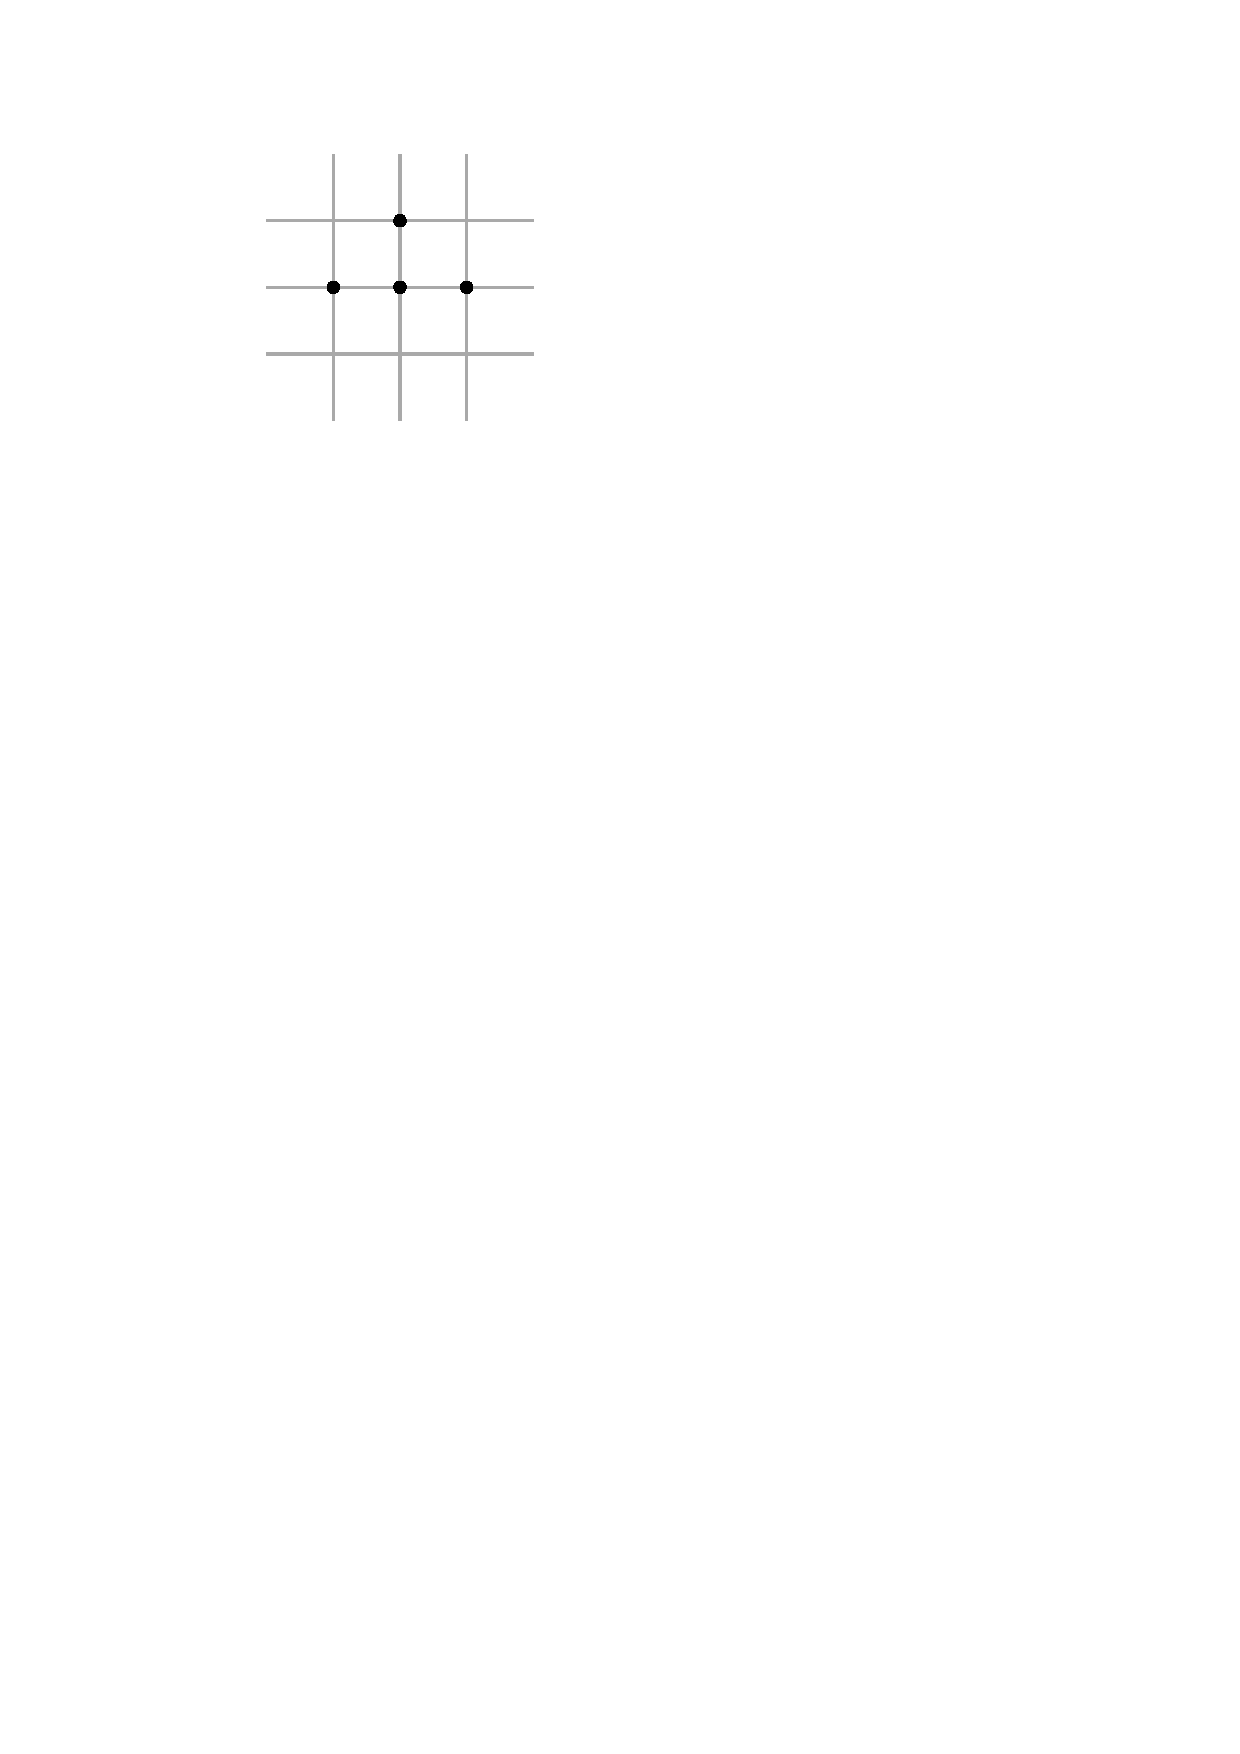
\includegraphics[scale=0.9]{../img/pde/therm-simple.pdf}
        \end{center}
        \caption{Простейшая явная схема для уравнения теплопроводности.}
    \end{figure}

    В таком виде уравнения можно писать для $i \in 1\ldots n-1$, $k\in 0\ldots M-1$; нужны дополнительные с граничными условиями. 

    \begin{itemize}
        \item Начальные условия: $u_i^0 = \varphi(x_i)$.
        \item Граничные условия:
        \begin{enumerate}
            \item $u_0^k = \alpha_1(t_k)$, $u_n^k = \alpha_2(t_k)$; при этом выполняются условия согласования \ti{нулевого порядка}
            \[
                \varphi(a) = \alpha_1(0), \quad \varphi(b) = \alpha_2(0).
            \]
            \item Для типов II, III используются такие же трюки, как в обычных диффурах. Надо аппроксимировать производные. Можно применять метод фиктивных точек или метод исключения главного члена погрешности.

            В угловых точках снова возникнет два разных условия:
            \[
                u_0^0 = \varphi(a) \text{ и } \dfrac{\pd u}{\pd x}(a, \, 0) = \beta_1(0) u_0^0 + \alpha_1(0).
            \]
            Будет ли выполняться равенство
            \[
                \varphi'(a) = \beta_1(0) u_0^0 + \alpha_1(0)?
            \]
            Оно называется \ti{условием согласования I порядка}. Без него уравнения не станут формально противоречивы.
        \end{enumerate}
    \end{itemize}

    Если разрешить уравнения относительно $u_i^{k + 1}$, получится 
    \[
        u_{i}^{k + 1} = A_i^k u_{i-1}^k + B_i^k u_i^k + C_i^k u_{i+1}^k + D_i^k.
    \]
    Коэффициенты выражаются по формулам
    \[
        \begin{array}{ll}
            A_i^k = \sigma a_0 - \sigma a_1 \dfrac{h}{2}, & C_i^k = \sigma a_0 + \sigma \dfrac{h}{2} a_1, \\
            B_i^k = 1 - 2 \sigma a_0 + \tau a_2,  &D_i^k = \tau f(x_i, \, t_k),
        \end{array}
    \]
    где $\sigma = \dfrac{\tau}{h^2}$.

    Можно просто двигаться вперёд по \ti{слоям}~--- множествам точек с постоянным временем; значения находятся последовательно.

    \paragraph{Неявная схема для уравнения теплопроводности}

    Неявная схема получается, если в \ref{eq:therm-A-B} выбрать вариант B. Сверху вниз (т.е. назад по времени) просчитать не получится, поскольку начальные данные даются в начале, а не в конце.

    \begin{figure}[h] \label{fig:therm-implicit}
        \begin{center}
            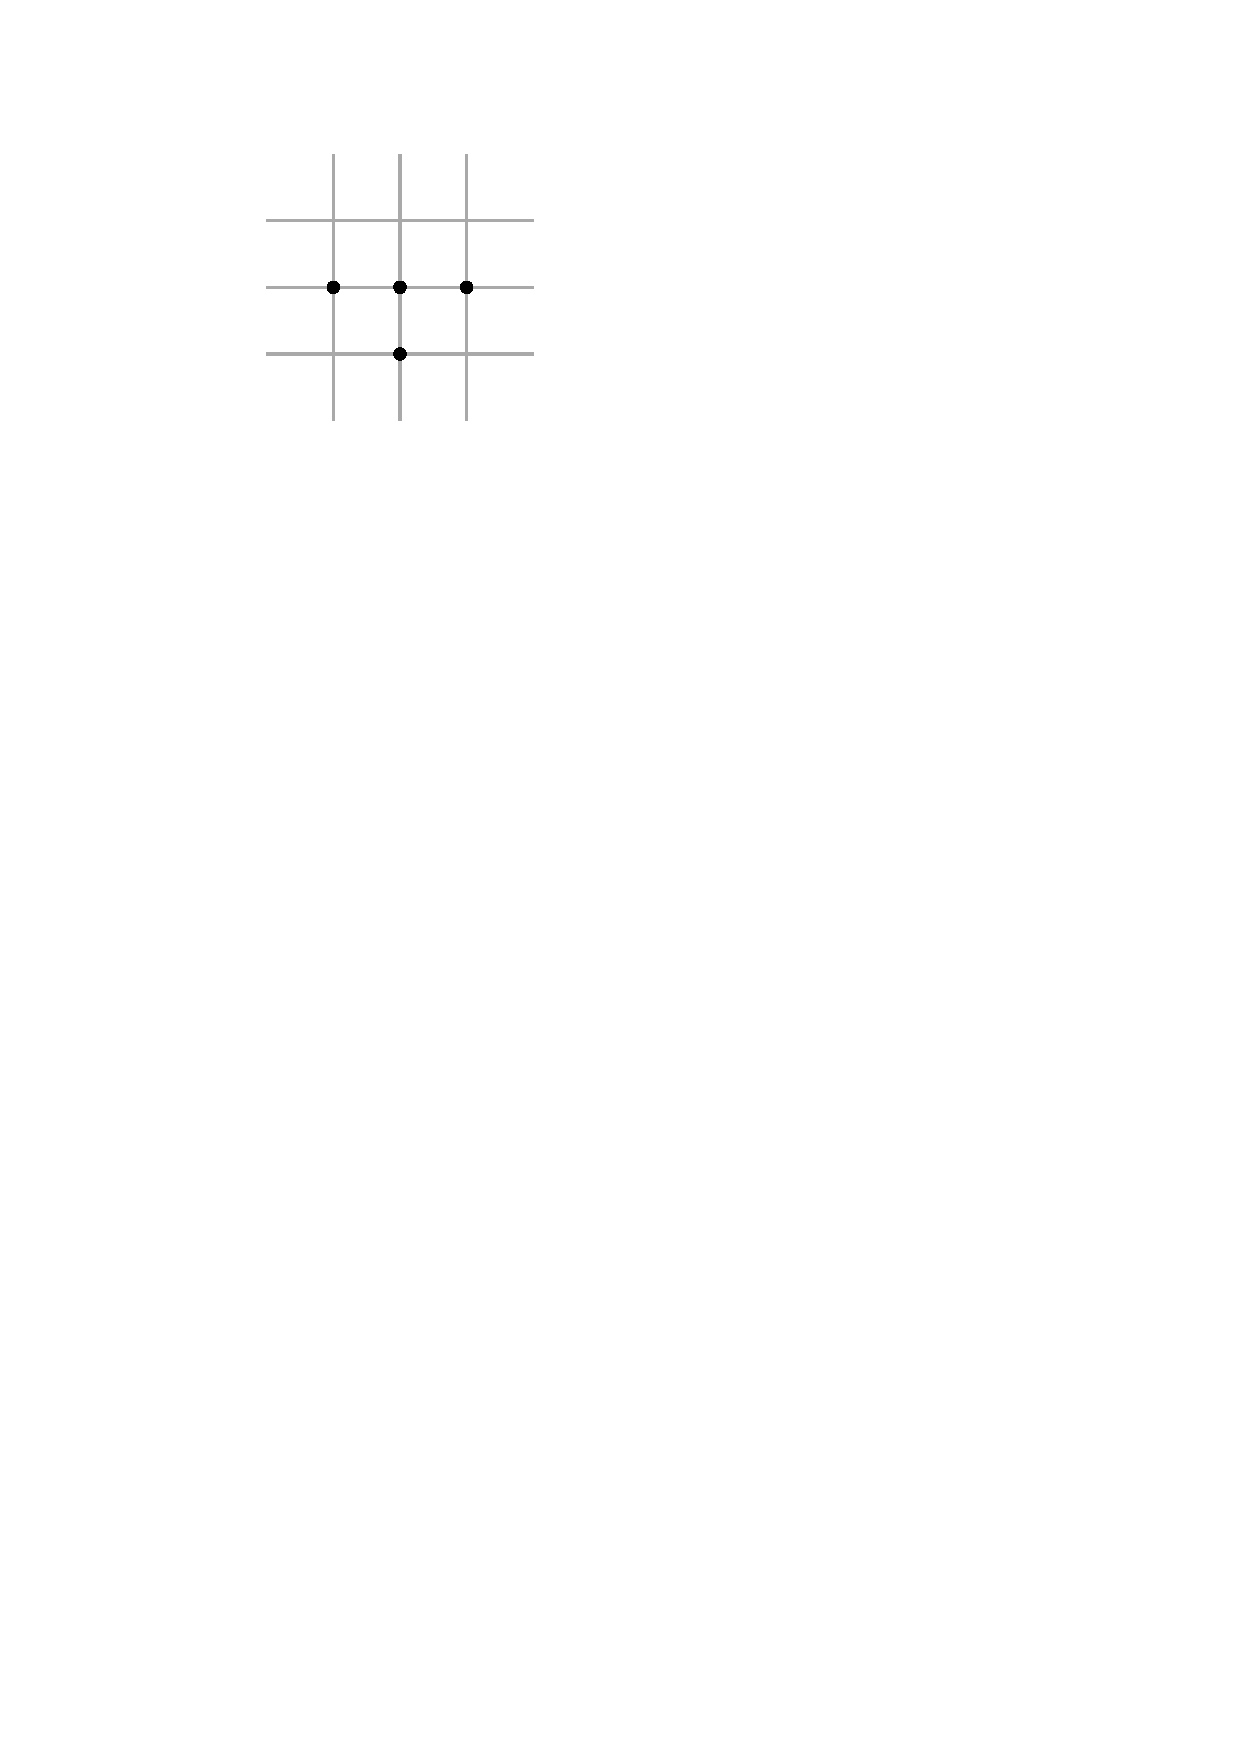
\includegraphics[scale=0.9]{../img/pde/therm-implicit.pdf}
        \end{center}
        \caption{Неявная схема для уравнения теплопроводности.}
    \end{figure}

    Формулы получатся такие:
    \[
        A_i^k u_{i-1}^k - B_i^k u_i^k + C_i^k u_{i+1}^k = D_i^k,
    \]
    где
    \[
        \begin{array}{ll}
            A_i^k = \sigma a_0 - \sigma a_1 \dfrac{h}{2}, & C_i^k = \sigma a_0 + \sigma \dfrac{h}{2} a_1, \\
            B_i^k = 1 + 2 \sigma a_0 - \tau a_2,  &D_i^k = -u_i^{k-1} - \tau f(x_i, \, t_k),
        \end{array}
    \]
    и $\sigma = \dfrac{\tau}{h^2}$.

    По сути, движение всё ещё послойное. Но на каждом слое я не могу просто посчитать значение, используя три значения с предыдущего слоя: наоборот, получается уравнение, которое связывает три значения с текущего слоя с одним уже известным. В итоге получается система с трёхдиагональной матрицей, которая замыкается добавлением граничных условий:
    \[
        u_0^k = \alpha_1(t_k), \; u_n^k = \alpha_2(t_k),
    \]
    если они заданы по первому типу, в противном случае применяются стандартные аппроксимации. 

    Система решается методом разностной прогонки \ref{par:ode::fintdma}.

    %unsure
    Кажется, тут утверждается, что метод прогонки срабатывает, поскольку
    \[
        A_i^k + C_i^k = 2\sigma a_0 = B_i^k + \tau a_2 - 1,
    \]
    и можно сослаться на \ref{prop:ode::diffeqest::suff}. Наверное, на практике это правда так, потому что $\tau a_2 \ll 1$, но выглядит сомнительно, я чего-то не понял.
    %unsure

    \paragraph{Явная схема для простейшего уравнения теплопроводности, решение разностных уравнений, неустойчивость}

    Рассмотрим уравнение
    \[
        \dfrac{\pd u}{\pd t} = \dfrac{\pd^2 u}{\pd t^2}, \quad t \in [0, \, \pi].
    \]
    с начальным условием $u(x, \, 0) = \varphi(x)$ и граничными условиями
    \[
        u(0, \, t) = u(\pi, \, t) = 0
    \]

    Для него разностные уравнения исключительно просты:
    \[
        \dfrac{u^{k + 1}_l - u^k_l}{\tau} = \dfrac{u^k_{l + 1} - 2u^k_l + u^k_{l-1}}{h^2}, \quad u_0^k = u_n^k = 0.
    \]
    При этом
    \[
        h = \dfrac{\pi}{n}, \quad x_l = lh, \quad u_l^0 = \varphi(x_l).
    \]

    Решим наше разностное уравнение методом разделения переменных, будем искать решение в виде
    \[
        u_l^k = \lambda^k e^{imx}, \quad x = x_l = lh.
    \]
    Подставим:
    \[
        \dfrac{\lambda^{k + 1}e^{imx} - \lambda^{k}e^{imx}}{\tau} = \dfrac{\lambda^k e^{im(x+h)} - 2\lambda^k e^{imx} + \lambda^k e^{im(x-h)}}{h^2}.
    \]
    Несложными выкладками отсюда находится
    \[
        \lambda = 1 + 2\sigma \big(\cos mh - 1\big)\,, \quad \sigma = \dfrac{\tau}{h^2}.
    \]
    Но такое решение не удовлетворяет граничным условиям; можно рассмотреть какую-нибудь комбинацию решений! Заметим, что $\lambda(m)$~--- чётная функция, поэтому 
    \[
        \lambda^k(m) \big(e^{imx} - e^{-imx}\big) = 2i\lambda^k(m)\sin(mx)
    \]
    тоже решение. Оно удовлетворяет граничным условиям при целых $m$; в итоге получаем
    \[
        \boxed{u_l^k = \lambda^k(m) \cdot \sin (mx), \quad m \in \Z}\,.
    \]
    У нас теперь есть $n-1$ ЛНЗ решение, из которых можно собирать новые:
    \[
        \varphi(x) = \sum\limits_{m = 1}^{n - 1} C_m \lambda^k(m) \cdot \sin (mx).
    \]

    \begin{rem}
        Остальные значения $m$ нам не интересны, поскольку у нас набралась $n-1$ базисная функция: действительно, изначально наши разностные уравнения решались однозначно, а сейчас мы их решили, учитывая граничные условия, но отпустив начальные. А их как раз $n - 1$~--- от $u^0_1$ до $u^0_{n-1}$, они и создают все степени свободы.
    \end{rem}

    Рассмотрим $\tau = h^2 \so \sigma = 1$:
    \[
        \lambda(m) = -1 + 2 \cos mh.
    \]
    При $m = n - 1$ и густой сетке (большом $n$)
    \[
        \cos \dfrac{(n - 1)\pi}{n} = \cos \left(\pi - \dfrac{\pi}{n}\right) \approx -1 \so \lambda(n - 1) \approx -3!
    \]

    При увеличении $k$ решение
    \[
        (-3)^k \sin(n - 1)x
    \]
    очень быстро растёт по модулю и всё время меняет знак. Кажется, что-то пошло не так!

    \begin{rem}
        Реальное решение такой задачи~--- быстро убывающая колебашка. Конечно, пространственный шаг взят большим: у начальных данных есть переменность на том же масштабе. Однако то, что при уменьшении шага по времени $k$ получает возможность становиться больше, уже вообще ни в какие ворота не лезет.
    \end{rem}

    %unsure
    %когда говорят про устойчивость, имеют в виду схему с фиксированным \tau или нет?
    %unsure

    Чтобы решения не вымирали подобным образом, можно наложить ограничение $|\lambda| \leqslant 1$:
    \[
        1 + 2\sigma \big(\cos mh - 1\big) \leqslant 1 \so 2\sigma \cos mh - 1 \leqslant 0 \so 2 \sigma \cos mh \leqslant 1.
    \]
    Чтобы это выполнялось при любых $m$, нужно, чтобы
    \[
        \boxed{\sigma \leqslant \dfrac{1}{2} \eqv \tau \leqslant \dfrac{h^2}{2}} \, .
    \]

    Если точно так же решить разделением переменных систему уравнений для простейшей неявной схемы, получим
    \[
        \lambda = \dfrac{1}{1 + 2\sigma(1 - \cos mh)} \leqslant 1,
    \]
    и устойчивость всегда присутствует.

    \paragraph{Общее определение устойчивости, теорема об устойчивости и сходимости}

    В начале книги \cite{gavurin} есть общие рассуждения про вычислительные методы и всякие пространства. В книге \cite{comp-krilov-2} есть про устойчивость, аппроксимацию, сходимость, их связь между собой, и про схемы для уравнения теплопроводности.

    С какой ситуацией мы сталкиваемся, занимаясь сеточными методами? У нас есть оператор $A\col \; U \to F$, и мы решаем уравнение вида
    \[
        Au = f.
    \]
    Выбирая сетку с шагом $h$ на отрезке, мы вместо функций на отрезке начинаем рассматривать функции на самой сетке~ они образуют другое, гораздо более маленькое пространство $U_h$. При этом по любому элементу $U$ можно легко найти элемент $U_h$, просто вычислив его значения на сетке. Аналогично строится пространство $F_h$\footnote{Зачастую $U_h = F_h$ и даже $U = F$, но может быть и не так, в принципе~--- вдруг, например, оператор действует в пространство функций на другом отрезке, или просто там другие ограничения на гладкость/непрерывность.}.

    Наконец, есть оператор $A_h \col \; U_h \to F_h$~--- приближение $A$, которое получается при переходе к конечным разностям. Для иллюстрации полезна диаграмма
    \[
        \xymatrix{
            U \ar@{->}[r]^{A} \ar@{->}[d]_{\varphi_h} & F \ar@{->}[d]^{\psi_h} \\ U_h \ar@{->}[r]^{A_h} & F_h
        }
    \]
    \begin{de}
        Операторы $\varphi_h(u)(x_l) = u(x_l)$ и такой же $\psi_h$ называются \ti{операторами (простого) сноса}.
    \end{de}

    \begin{rem}
        Понятно, что диаграмма должна быть почти коммутативна, но не совсем: если мы сначала продифференцируем функцию, а потом возьмём результат на сетке, и если мы сначала возьмём её на сетке, а потом посчитаем разностный аналог производной, получатся близкие, но разные вещи. Разность
        \[
            A_h\varphi_h(u) - \psi_h(Au)
        \]
         называется \ti{естественной погрешностью метода}.
    \end{rem}

    Далее, записывается разностное уравнение
    \[
        A_h \tilde{u} = \psi_h(f)
    \]
    и решается.

    Во всех четырёх пространствах надо ввести нормы. В пространствах функциональной природы $U$, $F$ они уже и так есть, вероятно.

    \begin{de}
        Говорят, что норма на $U_h$ \ti{согласована} с нормой на $U$, если верно, что 
        \[
            \|\varphi_h u\|_{U_h} \to \|u\|_U,
        \]
        когда $h \to 0$ хотя бы для $u \in K \subset U$, где $K$ плотно в $U$.

    \end{de}

    Будем считать, что у нас нормы согласованы.

    \begin{de}
        Говорят, что $A_h$ \ti{аппроксимирует} $A$ на $u \in U$, если 
        \[
            \big\|A_h\varphi_h(u) - \psi_h(Au)\big\| \to 0 \text{ при } h \to 0.
        \]
    \end{de}

    \begin{de}
        Говорят, что сеточные функции $u_h$ сходятся к функции $u \in U$, если 
        \[
            \big\|u_h - \varphi_h(u)\big\| \to 0 \text{ при } h \to 0.
        \]
    \end{de}

    \begin{de}
        Говорят, что \ti{сеточное приближение} обладает \ti{свойством аппроксимации}, если $A_h$ аппроксимирует $A$, и сеточные функции $f_h$ сходятся к $f$.
    \end{de}

    \begin{de}  
        Говорят, что сеточное приближение \ti{устойчиво}, если
        \begin{enumerate}
            \item Уравнение $A_hu_h = f_h$ однозначно разрешимо для всех $f_h \in F_h$;
            \item Для этого решения $\|u_h\| \leqslant k \|f_h\|$, где $k$ не зависит от $h$.
        \end{enumerate}
    \end{de}

    \begin{thm}[Основная теорема теории разностных методов]
        Пусть дана некоторая краевая задача, и сеточная аппроксимация удовлетворяет следующим свойствам:
        \begin{enumerate}
            \item $u^*$~--- единственное решение уравнения $Lu^* = f$.
            \item Сеточное приближение обладает свойством аппроксимации.
            \item Сеточная задача устойчива.
        \end{enumerate}
        Тогда есть сходимость сеточных решений: $u^*_h \to u$.
        \begin{proof}
            Запишем ошибку сеточного решения:
            \[
                w_h = u_h^* - \varphi_h u^*.
            \]
            Заметим, что по свойству устойчивости
            \begin{align*}
                \|w_h\| &\leqslant k \|L_h w_h\| = k\|L_h u_h^* - L_h \varphi_h u^*\| = \\ &= k\|f_h - \psi_h f + \psi_h f - L_h \varphi_h u^*\| \leqslant k\|f_h - \psi_h f\| + k\|\psi_h L u^* - L_h \varphi_h u^*\|.
            \end{align*}
            Оба слагаемых в правой части стремятся к нулю по свойству аппроксимации.
        \end{proof}
    \end{thm}

    \paragraph{Разностные схемы для задач с начальными условиями, дискретное преобразование Фурье}

    \begin{rem}[\textbf{DISCLAIMER}]
        ПРОИЗОШЛО СЖАТИЕ С ПОТЕРЯМИ ШАКАЛОМЕТР ЗАШКАЛИВАЕТ БИП 
    \end{rem}

    В этом параграфе в целом посмотрим на уравнение 
    \[
        \dfrac{\pd u}{\pd t} = Lu + f,
    \]
    где всё многомерное (т.е. $u$~--- вектор, а $L$~--- <<матрица>> из частных производных), и $L$~--- линейный дифференциальный оператор с постоянными коэффициентами. Область определения $u$~--- цилиндр $D\times [0, \, T] \subset \R^{p + 1}$. Начальные условия~--- $u(x, \, 0) = \varphi(x)$.

    Ограничимся теперь ситуацией, когда $D$~--- куб $[0, \, 2\pi]^p$, а граничные условия периодические по каждой из переменных (т.е. $u(x_1, \ldots, \, 0, \ldots, \, x_p; \, t) = u(x_1, \ldots, \, 2\pi, \ldots, \, x_p; \, t)$). 

    По каждой из пространственных переменных выберем одинаковые шаги
    \[
        h = \dfrac{2\pi}{N},
    \] 
    а по временной~--- шаг
    \[
        \tau = \dfrac{T}{M}.
    \]
    По пространственной причём рассматриваем только от $0$ до $M-1$, потому что справа снова будет то же граничное значение. Уравнения будут двухслойными, с $k$-го и $k+1$-го слоя.

    Даже в неявном случае с помощью разностной прогонки можно выразить все следующие слои через предыдущие и получить уравнения
    \[
        u_h(k + 1) = R_h u_h(k) + \rho_h(k),
    \]
    где $R_h$~--- \ti{оператор перехода в однородном случае}. $R_h$~--- просто матрица с постоянными коэффициентами, а $\rho_h(k)$ зависит от $f$.

    \begin{rem}
        Всё-таки скажу про эти обозначения пространств... $V_h$~--- пространство сеточных функций \ti{на фиксированном слое} (т.е. оно $N$-мерное), а $F_h$~--- видимо, аналогичное пространство, которое мы отличаем только по формальным причинам, в котором лежат $f_h$~--- сеточные версии $f$. Нормы в обоих пространствах~--- просто $l^{\infty}$, т.е.
        \[
            \big\|\{u_i\}\big\| = \max |u_i|.
        \]
    \end{rem}

    \begin{thm} \label{thm:stab-1}
        Для устойчивости при $f = 0$ необходимо и достаточно, чтобы были ограничены $\|R_h^k\|$ (здесь $k$~--- степень!) при $k\tau \leqslant T$.
        \begin{proof}
            Оно в целом понятно: когда нет $f$-ок, нет и $\rho$-шек, а без них переход на следующий слой~--- тупо умножение на матрицу $R_h$. Ясно, что если нормы этих матриц в совокупности ограничены, то и
            \[
                \|u_h(k+1)\| \leqslant C \|\varphi\|,
            \]
            где $\varphi$ задаёт начальные условия.

            Обратно тоже понятно: если ограниченности норм матриц нет, можно просто пойти от противного и сконструировать мерзкую последовательность.
        \end{proof}
    \end{thm}

    \begin{thm}
        Если $f \neq 0$ и $\|R_h^k\|$ ограничены, то для устойчивости достаточно, чтобы
        \[
            \|\rho_h\|_{V_h} \leqslant c_2 \tau \|f_h\|_{F_h}
        \]
        \begin{proof}
            Обычная оценка, см. конспект Ангелины, страница 75.
            %unsure
        \end{proof}
    \end{thm}

    \begin{cor}
        Если $\|R_h\| \leqslant 1 + c_3\tau$, то есть устойчивость (при $f = 0$).
        \begin{proof}
            \[
                \|R_h^k\| \leqslant \|R_h\|^k \leqslant (1 + c_3 \tau)^k \leqslant e^{c_3 \tau k} \leqslant e^{c_3 \tau}.
            \]
        \end{proof}
    \end{cor}

    По поводу этих теорем можно ещё заглянуть в следующий параграф \ref{par:neumann}, там доказаны очень похожие вещи.

    Перейдём теперь к дискретному преобразованию Фурье. Пусть размерность $p$ пока равна $1$. Введём на пространстве $V_h$ функций на фиксированном слое скалярное произведение:
    \[
        (u_h, \, v_h) = h \sum\limits_{i = 0}^{N - 1} u_h \ov{-}{v_h}
    \]

    \begin{st}
        Набор функций $e_m(x) = e^{imx}$, где $m \in 0\ldots N-1$, образует ортогональный базис в $V_h$, причём
        \[
            (e_m, \, e_m) = 2\pi.
        \]
        \begin{proof}
            Чтобы увидеть, что они ортогональны, достаточно посчитать скалярное произведение. Отсюда следует, в принципе, что они ЛНЗ. Ну а дальше~--- их $N$, пространство $N$-мерное, потому и базис.
        \end{proof}
    \end{st}

    \begin{de}
        \ti{Обратное дискретное преобразование Фурье}~---
        \[
            \{a_1, \, \ldots, \, a_N\} \mapsto \sum\limits_{i = 1}^{N-1} a_i e_i(x).
        \]
        \ti{Прямое ДПФ}~---
        \[
            u_h \mapsto \dfrac{1}{2\pi}\big\{(u_h, \, e_1), \ldots, \, (u_h, \, e_n)\big\}.
        \]
        Ясно, что это взаимно обратные операторы.
    \end{de}

    \begin{st}[Формула замкнутости]
        Дискретное преобразование Фурье~--- почти унитарный оператор, т.е. 
        \[
            \left(\sum\limits_{i = 1}^{N - 1} a_i e_i, \; \sum\limits_{i = 1}^{N - 1} b_i e_i\right) = 2 \pi \sum_{i = 0}^{N - 1} a_i \ov{-}{b_i}.
        \]
        \begin{proof}
            Проверяется прямым вычислением.
        \end{proof}
    \end{st}

    \begin{st}
        $e^{imx}$~--- собственная функция оператора сдвига
        \[
            T_h u(x) = u(x + h)
        \]
        с собственным числом $e^{imh}$.
        \begin{proof}
            Действительно,
            \[
                T_h e^{imx} = e^{im(x + h)} = e^{imh} e^{imx}.
            \]
        \end{proof}
    \end{st}

    \begin{rem}
        У нас периодические граничные условия, поэтому оператор сдвига может действовать, <<переходя>> через границу:
        \[
            T_h \{u_0, \, \ldots, \, u_{N - 1}\} = \{u_{1}, \, u_2, \, \ldots, \, u_{N-1}, \, u_0\}.
        \]
        Можно представлять себе, что индекс $i$ на самом деле меняется от $-\infty$ до $\infty$, но $u_{i + N} = u_i$. Периодическую функцию можно восстановить, зная её значения внутри периода, вот и здесь так же.
    \end{rem}

    \begin{rem}
        В такой ситуации любой разумный разностный оператор можно собрать из операторов сдвига. Например, пусть
        \[
            (Du)_i = \dfrac{u_{i + 1} - 2u_i + u_{i - 1}}{h}.
        \]
        Это можно переписать просто как
        \[
            Du = \dfrac{T_hu - 2u + T_{-h}u}{h}.
        \]
        Общая формула, естественно, будет такая:
        \[
            Lu = \sum\limits_{\alpha} c(\alpha) T_h^{\alpha}(u),
        \]
        где $\alpha \in \Z$~--- показатель степени.

        Тем удобнее будет применять эти операторы к экспонентам~--- от них ведь сдвиг считать легко.
    \end{rem}

    Это всё можно написать и в многомерии, при $p>1$, но, кажется, У Оли этого нет. См. конспект Ангелины, билет и так длинный.

    Применим теперь построенную теорию к сеткам. Сеточное уравнение будет выглядеть примерно так:
    \[
        \sum\limits_{\alpha \in A_0} A(\alpha) u(x + \alpha h, \, k \tau) = \sum\limits_{\beta \in B_0} B(\beta) u\big(x + \beta h, \, (k+1) \tau\big).
    \]
    Ну, это просто два слоя, $k$-й и $k+1$-й. Теперь сделаем ДПФ, пусть
    \[
        u(x, \, k\tau) = \sum a^k(m) e^{imx}.
    \]
    Подставим это в суммы:
    \[
        \sum\limits_{\alpha \in A_0} e^{im\alpha h} A(\alpha) \sum\limits_m a^k(m) e^{imx} = \sum\limits_{\beta \in B_0} e^{im\beta h} B(\beta) \sum\limits_m a^{k+1}(m) e^{imx}.
    \]
    Слева и справа написаны два разложения по базису, коэффициенты в которых должны совпадать:
    \[
        a^k(m) \sum\limits_{\alpha \in A_0} e^{im\alpha h} A(\alpha)  = a^{k+1}(m) \sum\limits_{\beta \in B_0} e^{im\beta h} B(\beta) 
    \]
    В итоге получаем
    \[
        a^{k + 1}(m) = c(m) a^k(m), \quad c(m) = \dfrac{\sum\limits_{\alpha \in A_0} e^{im\alpha h} A(\alpha)}{\sum\limits_{\beta \in B_0} e^{im\beta h} B(\beta)}.
    \]

    \paragraph{Необходимое условие устойчивости по фон Нейману}\label{par:neumann}

    \begin{rem} 
        %unsure
        Коэффициент $c$~--- по сути, видимо, диагональная матрица. Это матрица перехода между слоями в терминах коэффициентов Фурье. 

        Я не совсем понял, где в конспекте проходит грань между матрицей и числом (всё усложняется тем, что в высших размерностях $m$~--- мультииндекс, а $u^k$ и $c$, видимо, <<тензоры>>). Поэтому я буду исходить из того, что $c(m)$~--- просто число, а $c$~--- набор этих чисел, причём
        \[  
            \|c\| = \|c\|_{l^{\infty}} = \max\limits_m c(m).
        \]
        Ну и вообще, пусть все доказательства будут одномерными.
        %unsure
    \end{rem}

    \begin{thm}
        Для устойчивости при $f = 0$ необходимо и достаточно, чтобы
        \[
            \|c^k\| \leqslant c_3, \quad k\tau \leqslant T.
        \]
        \begin{proof}
            Интересно, видимо, доказывать достаточность. Попробуем просто найти оценку на норму $u_h(k)$.
            \[
                a(k, \, m) = c^k(m)a(0, \, m),
            \]
            поэтому 
            \[
                u_h(k) = \sum\limits_m a(k, \, m) e^{imx} = \sum\limits_m a(0, \, m) c^k(m) e^{imx}.
            \]
            Далее $K$~--- произвольная неотрицательная константа, в которую можно вносить другие.
            По формуле замкнутости
            \begin{align*}
                \big\|u_h(k)\big\|_{l^2}^2 &= 2\pi \sum\limits_m \big|a(0, \, m) c^k(m)\big|^2 \leqslant \\ & \leqslant K \max\limits_{m} \big|a(0, \, m)\big|^2 \big|c^k(m)\big|^2 \leqslant  K \max\limits_m |a(0, \, m)\big|^2.
            \end{align*}
            Последний переход возможен, поскольку $\|c^k\| \leqslant c_3$.
            При этом
            \begin{align*}
                \max\limits_m |a(0, \, m)\big|^2 &= \left(\max\limits_m |a(0, \, m)\big|\right)^2 = \|a^0\|_{l^{\infty}}^2 \leqslant \\ &\leqslant K\|a^0\|_{l^2}^2 = K \big\|u_h(0)\big\|_{l^2}^2 \leqslant K\big\|u_h(0)\big\|_{l^{\infty}}^2.
            \end{align*}
            В итоге получаем
            \[
                \big\|u_h(k)\big\|_{l^{\infty}}^2 \leqslant K\big\|u_h(k)\big\|_{l^2}^2 \leqslant K\big\|u_h(0)\big\|_{l^{\infty}}^2.
            \]
            Это и есть устойчвость, по сути.
            Чтобы доказать необходимость, предположим, что нет такой оценки $\|c^k\| \leqslant c_3$, не зависящей от $h$ и $\tau$. Рассмотрим $u_h(0) = e^{imx}$. Тогда
            \[
                a(0, \, l) = \delta_{ml} \so u_h(k) = c^k(m)e^{imx}.
            \]
            По предположению мы можем так подобрать $h, \, \tau, \, m, \, k$, что $\big|c^k(m)\big|$ станет сколь угодно большим; но тогда это произойдёт и с $\|u_h(k)\|$! Понятно, что никакой устойчивости нет и в помине.
        \end{proof}
    \end{thm}

    \begin{thm}[условие фон Неймана]
        Для устойчивости при $f = 0$ необходимо и достаточно, чтобы собственные числа $c$ удовлетворяли условию
        \[
            |\lambda| \leqslant 1 + c_4 \tau.
        \]
        \begin{proof}
            Ну, достаточность не слишком сложна:
            \[
                \|c^k\| = \max \limits_m \big|c(m)\big|^k \leqslant \big|1 + c_4 \tau\big|^k \leq e^{kc_4\tau} \leqslant e^{c_4 T}.
            \]
            Необходимость, впрочем, тоже. Пусть этого условия нет; тогда для любого $c_4$ можно подобрать такие $h$, $\tau$ и $m$, что $c(m) > 1 + c_4\tau$. Но тогда 
            \[
                \|c^k\| \geqslant \big|c(m)^k\big| \leqslant (1 + c_4 \tau)^k.
            \]
            Ясно, что увеличивая $c_4$, можно неограниченно увеличивать $\|c^k\|$.
        \end{proof}
    \end{thm}

    \begin{rem} 
        Кажется, в многомерии это условие только необходимое, но я не очень понимаю, почему.
    \end{rem}



\end{document}


\clearpage

\appendix
\chapter{Введение в функциональный анализ}
\documentclass{trlnotes}
\setlayout{hardcopy}
\usepackage{silence}
\WarningFilter{latex}{Reference}
\graphicspath{{../../img/}}

\begin{document}
    \paragraph{Пространства, отображения}
    Бесконечномерные пространства во многом похожи на конечномерные, но есть и различия. Приведём наглядный пример:

    \begin{thm}(Рисса)
        В бесконечномерном пространстве с нормой единичный замкнутый шар не компактен. \footnote{Верно и обратное утверждение: если в нормированном пространстве единичный замкнутый шар компактен, то оно конечномерно.}
        \begin{proof}
            Чтобы доказать, что что-то не компактно, нужно найти там последовательность, у которой нет сходящейся подпоследовательности. Здесь это нетрудно: подойдёт любой счётный ортнормированный набор векторов!

            Представьте себе: у вас есть $n$ единичных ортогональных друг другу векторов. Вы можете добавить ещё один, и ещё, и ещё... Конечно, в такой последовательности не выбрать сходящейся.
        \end{proof}
    \end{thm}

    В том, что касается линейных отображений, тоже есть тонкости. Мы знаем, что любое линейное отображение конечномерных пространств непрерывно и \ti{ограничено} (т.е. образ единичного замкнутого шара при нём ограничен). В бесконечномерном случае это не так! Однако выполняется такое утверждение:

    \begin{st}
        Для нормированных пространств непрерывность и ограниченность линейных отображений равносильны.
    \end{st}

    В реальности почти все интересные отображения ограничены. Да и у неограниченных слишком плохие свойства, поэтому в большинстве теорем ограниченность предполагается.

    \paragraph{Спектр оператора}

    Ещё одно различие, не столь наглядное, но очень важное, связано со \ti{спектром} оператора.

    \begin{de}
        Пусть $H$~--- гильбертово пространство, $A\col \; H \to H$~--- ограниченный оператор. \ti{Спектром} $A$ называют множество таких $\lambda \in \C$, что оператор $A - \lambda I$ необратим.
    \end{de}
    Понятие спектра тесно связано с собственными числами:
    \begin{de}
        Говорят, что $\lambda \in \C$~--- \ti{собственное число} оператора $A$, если есть такой вектор $v \in H$, что $Av = \lambda v$.
    \end{de}
    Собственные числа можно охарактеризовать в терминах оператора $A - \lambda I$:
    \begin{st}
        $\lambda$~--- собственное число $A$ тогда и только тогда, когда оператор $A - \lambda I$ не инъективен (то есть склеивает какие-то векторы в один).
        \begin{proof}
            Пусть $\lambda$~--- собственное число, $v$~--- собственный вектор. Тогда $(A - \lambda I)v = 0 = A0$, поэтому оператор не инъективен.

            Докажем в обратную сторону. Пусть оператор $A - \lambda I$ не инъективен. Тогда есть вектор из ядра~--- такой, что $(A - 
            \lambda I)v = 0$, т.е. $Av = \lambda v$.
        \end{proof}
    \end{st}

    Отсюда сразу следует утверждение:
    \begin{st}
        Для конечномерных пространств спектр и множество собственных чисел~--- одно и то же.
        \begin{proof}
            Как мы знаем,
            \[
                \text{необратимость} \eqv \text{неинъективность или несюръективность}.
            \]
            Но в конечномерном случае 
            \[
                \text{несюръективность} \so \text{неинъективность}.
            \]
            Это связано с тем, что несюръективный оператор понижает размерность пространства, что вынуждает его склеивать вектора.

            Поэтому необратимость либо сразу влечёт неинъективность, либо сначала влечёт несюръективность, а потом уже неинъективность. Отсюда
            \[
                \text{необратимость} \eqv \text{неинъективность},
            \]
            что и требовалось доказать.
        \end{proof}
    \end{st}

    В бесконечномерном случае всё не так. Из необратимости неинъективность больше не следует, и у оператора появляются два разных способа быть необратимым:

    \begin{enumerate}
        \item Оператор склеивает векторы.
        \item Образ оператора меньше, чем всё пространство.
    \end{enumerate}

    Поэтому спектр оператора $A$ в бесконечномерном пространстве разбивается на собственные числа и те точки, в которых $A - \lambda I$ не является сюръективным (хоть и векторы не склеивает). 

    \begin{rem}
        Это не мифическая ситуация: обычный оператор умножения на координату (т.е. $Af(x) = x f(x)$) в $L^2\big([a, \, b]\big)$ не имеет собственных чисел, но его спектр равен всему отрезку! 

        Когда мы занимались квантовой механикой, мы находили <<собственные вектора>>~--- дельта-функции. То, что они на самом деле не функции и в $L^2$ не лежат~--- свидетельство описанного феномена!
    \end{rem}

    \paragraph{Компактные операторы}

    Обсудим один класс операторов, очень полезный на практике.

    \begin{de}
        Пусть $H$~--- гильбертово пространство, $B$~--- единичный замкнутый шар в нём. Оператор $A\col \; H \to H$ называют \ti{компактным}, если замыкание множества $A(B)$ компактно.
    \end{de}

    \begin{rem}
        На самом деле, компактный оператор переводит любое ограниченное множество в множество с компактным замыканием.
    \end{rem}

    Мы знаем, что даже единичный шар в $H$ не компактен. Это значит, что $A$~--- оператор с очень маленьким образом, он сжимает всё пространство во что-то крохотное! Это объясняет простоту (и близость к конечномерию) свойств компактных операторов.

    \begin{st}
        Если операторы $A_n$ компактны и $\|A_n - A\| \to 0$, то оператор $U$ компактен.
    \end{st}

    \begin{cor}
        Если операторы $A_n$ конечного ранга (т.е. их образы конечномерны), и $\|A - A_n\| \to 0$, то оператор $A$ компактен.
    \end{cor}

    Главный пример компактного оператора~--- \ti{интегральный оператор}.

    \begin{exm}
        Пусть $\square = [a, \, b] \times [a, \, b]$. Рассмотрим оператор $A$ на $L^2\big([a, \, b]\big)$, действующий по правилу
        \[
            Af(x) = \int\limits_a^b K(x, y) f(y) \, \mathrm{d}y,
        \]
        где $K \in L^2(\square)$. Такой оператор называют \ti{интегральным}, а функцию $K$ называют его \ti{ядром}. В принципе, вместо $L^2$ можно жить в $C$~--- пространстве непрерывных функций, но оно не гильбертово.   
    \end{exm}

    \begin{st}
        Интегральный оператор компактен.
        \begin{proof}[Почти доказательство]
            Разложим функцию $K$ по базису (так можно, правда):
            \[
                K(x, \, y) = \sum\limits_{n, \, m = 0}^{\infty} c_{nm} e_n(x) e_m(y).
            \]
            Рассмотрим последовательность интегральных операторов $A_N$ с ядрами
            \[
                K_N(x, \, y) = \sum\limits_{n, \, m = 0}^{N} c_{nm} e_n(x) e_m(y).
            \]
            Простым преобразованием находим, что
            \[
                A_N f(x) = \sum\limits_{n = 1}^N \left(\,\sum\limits_{m = 1}^N c_{nm} \int\limits_a^b e_m(y) f(y) \, \del y\right) e_n(x).
            \]

            Образ оператора $A_N$ находится внутри линейной оболочки векторов $e_1, \, \ldots, \, e_N$! Это значит, что наш оператор $A$ приближается операторами конечного ранга, а потому компактен.
        \end{proof}
    \end{st}

    \paragraph{Спектры компактных операторов}

    

\end{document}
% vim:wrapmargin=3


\chapter{Обозначения}
% %------------------------------------------------------------
% Description : Стандартные обозначения 
% Author      : taxus-d <iliya.t@mail.ru>
% Created at  : Sat Jan 14 17:39:43 MSK 2017
%------------------------------------------------------------
\documentclass[12pt,timbord]{longnotes}
\usepackage{tmath}
\usepackage{cussymb}
\usepackage{silence}
\WarningFilter{latex}{Reference}
\graphicspath{{../../img/}}


\begin{document}

\section*{Обозначения с лекции}
\begin{description}
  \item[$a:= b$]~--- определение $a$.
  \item[$\displaystyle \bigsqcup_k A_k$]~--- объединение дизъюнктных множеств.
  \item[$\alg$]~--- Алгебра множеств
  \item[$\ov-{A}$]~--- Замыкание $A$.
  \item[$A^c$]~--- $X \setminus  A$.
\end{description}

\section*{Нестандартные обозначения}

\begin{description}
  \item[\underdev]~--- ещё правится. Впрочем, относится почти ко всему.
  \item[$\square\cdots\blacksquare$]~--- начало и конец доказательства теоремы
  \item[$\blacktriangledown\cdots\blacktriangle$]~--- начало и конец доказательства более мелкого 
    утверждения
  \item[\sour]~--- кривоватая формулировка
  \item[\flame]~--- набирающему зело не нравится билет
  \item[\plholdev{что-то}]~--- тут будет \texttt{что-то}, но попозже
  \item[$a\intrng b$]~--- $[a;b]\cap \Z$
  \item[$\equiv$]~--- штуки эквивалентны. Часто используется в этом смысле в
    определениях, когда вводится два разных обозначения одного и того же
    объекта.
  \item[$\that$]~--- В кванторах, <<верно, что>>
  \item[$\alg_\sigma$]~--- Сигма-алгебра множеств
  \item[$f \colon A \leftrightarrow B$]~---биекция
\end{description}
\end{document}



% \printbibliography[
%   heading=bibintoc,
%   title={Использованная литература}
% ]

\end{document}

